\chapter{Groups}

\section{Definitions}
\begin{definition}
A \textbf{group} is a set $G$, equipped with a binary operation
$\cdot : G \times G \to G$ which satisfies the three following axioms:

\begin{enumerate}
    \item[\textbf{(G1)}] The operation $\cdot$ is \textbf{associative}. Specifically, $a \cdot (b \cdot c) = (a \cdot b) \cdot c$ for all $a, b, c
    \in G$

    \item[\textbf{(G2)}] There exists an element $e \in G$, known as the
    \textbf{identity} of $G$, such that $a \cdot e = a = e \cdot a$
    for all $a \in G$ 

    \item[\textbf{(G3)}] For each $a \in G$, there exists an element $a^{-1} \in G$, 
    known as the \textbf{inverse} of $a$, such that $a \cdot a^{-1} =
    a^{-1} \cdot a = e$. 
\end{enumerate}
In this case, we say that \textbf{$G$ is a group under $\cdot$}, and denote
this  as $(G, \cdot)$.
\end{definition}

\begin{remark}
    \begin{itemize}
        \item Note that in order to have a group, we require a set $G$, and
        a binary operation. Hence we cannot say ``the set $X$ is a group.'' This
        makes no sense, although as we will see, sometimes this is written
        when the operation is obvious or stated.
    
        \item
        It goes without really explicitly stating that 
        $\cdot$ must also be \textbf{closed}; that is, it
        cannot map elements anywhere outside of $G$. This is due to our 
        definition that $\cdot : G \times G \to G$. That is, the
        codomain, or range, is always within $G$.
    \end{itemize}
\end{remark}

\begin{definition}
    Let $G$ be a group. Suppose that, for any two $g, h \in G$
    we have 
    \[
        g \cdot h = h \cdot g  
    \]
    then $G$ is an \textbf{abelian} or \textbf{commutative} group.
\end{definition}

\textbf{Notation.} 
First observe that we use $\cdot$ in our definition of a group. This
is unfortunately the same notation used in modern-day numerical
multiplication (i.e., $5 \cdot 3 = 15$). Here, this is not the case;
it's just a placeholder for \textit{some} operator. You'll get used
to this as you go in group theory.

In group theory, we denote the multiplication of
group elements $g$ and $h$ as $g \cdot h$. However, if the operator
$\cdot$ is already understood, then we will just write $gh$. If there
is possibility for confusion (i.e., perhaps in a situation in where
there are \textit{two} operators in play) we will be more explicit and
clear about our operator. Buts for the most part we'll just write $gh$.
\\
\\
\noindent
\textbf{Example.} Consider the set $\mathbb{Z}$, and let the operator
on the elements of $\mathbb{Z}$ simply be standard addition. This is a
group, which we'll demonstrate by showing that this set equipped with
the addition operator
satisfy the three axioms.
\begin{description}
    \item[(1) Closed.] From elementary mathematics, we know that if
    $m, n \in \mathbb{Z}$ then $m + n \in \mathbb{Z}$. Thus this set
    is closed under addition.

    \item[(2) Associativity.] Observe that for any integers $n, m $
    and $p$, 
    \[
        n + (m + p) = (n + m) + p.
    \]
    This is just a basic fact of elementary arithmetic.

    \item[(3) Identity.] Observe that for any $n \in \mathbb{Z}$, 
    \[
        n + 0 = 0 + n = n.        
    \]
    Thus 0 is an appropriate choice of an identity. 

    \item[(4) Inverse.] Consider any $n \in \mathbb{N}$. Observe that 
    (1) $-n \in \mathbb{Z}$ and (2) 
    \[
        n + (-n) = (-n) + n = 0.
    \] 
    Thus every element has an inverse. Note we specified that $-n \in
    \mathbb{Z}$, as we wanted to emphasize that not only $-n$ exists,
    but $-n$ is \textit{in} our set $\mathbb{Z}$.    

\end{description}
With all three properties satisfied, we have that $\mathbb{Z}$ is a
group with addition. More generally, we'd say that $\mathbb{Z}$ is a
group under addition, and denote it as $(\mathbb{Z}, +)$.
\\
\\
{\color{Plum} 
Note that $\mathbb{Z}$ is not a group under multiplication. Suppose we
try to say it is one anyways. Then the most natural step is to first note that $1$
should be our identity. After all, for any $n \in \mathbb{Z}$, $1
\cdot n = n \cdot 1 = n$. If we then consider any $m \in \mathbb{Z}$,
what is the inverse of $m$? We'd need a $p \in
\mathbb{Z}$ such that 
\[
    m\cdot p = p\cdot m = 1.
\]
This has no solution if $m > 1$; for example, there is no integer $p$ 
such that $5 \cdot p = 1$. In fact, $p = \dfrac{1}{5}$, can only
satisfy this in the set of real numbers, but $\dfrac{1}{5}$ is not
in $\mathbb{Z}$. Thus $\ZZ$ is not a group under multiplication, but
it is a group under addition.
}

\textcolor{red}{We reiterate again that these two examples highlight the fact that a
group requires two things: a set, and a well-defined operator that
acts on the set.}
\\

It turns out that $\mathbb{Q}\setminus\{0\}$ (not including zero) is a group under
multiplication. Also, $\mathbb{R}$ is a group under multiplication and
a group under addition. We wont show this (it's not much work) and
will instead move onto more interesting examples which capture how
versatile the definition of a group really is. 

\noindent
\textbf{Example.}
Consider the set of $n \times n$ matrices with determinant 1 and entries in $\mathbb{R}$, where
the multiplication is standard matrix multiplication. This is
known as the \textbf{Special Linear Group} and is denoted
$SL_n(\mathbb{R})$. We'll show that this set is a group.
\begin{description}
    \item[(1) Closed.] First we need to check if this operation is
    closed. That is, for $A, B \in SL_n(\mathbb{R})$, is it true that
    $AB \in SL_n(\mathbb{R})$?

    We know products of $n \times n$ matrices give
    back $n \times n$ matrices. So the real question is, 
    if two matrices both have
    determinant 1, will their product necessarily be a matrix
    whose determinant is also 1? 
    The answer is yes. From linear algebra, we know that 
    \[
        \det(AB) = \det(A)\det(B).
    \]
    Now if $A, B$ have determinant 1, 
    \[
        \det(AB) = \det(A)\det(B) = 1 \cdot 1 = 1.   
    \]
    Therefore, $AB \in SL_n(\mathbb{R})$, since $AB$ is $n \times n$
    and it has determinant 1.


    \item[(2) Associativity.] For matricies $A, B, C \in
    SL_n(\mathbb{R})$, we know from linear algebra that 
    \[
        (AB)C = A(BC).
    \]
    That is, matrix multiplication is associative.

    \item[(3) Identity.] Naturally, the identity matrix $I$ serves as
    our group identity. This is because for any $A \in
    SL_n(\mathbb{R})$, $AI = IA = A$.

    \item[(4) Inverses.] For any $A \in SL_n(\mathbb{R})$, $\det(A) =
    1$. Specifically observe that $\det(A) \ne 0$. Therefore by the 
    invertible matrix theorem, $A$
    has an inverse element $A^{-1}$ such that $AA^{-1} = A^{-1}A = I$.
    But the real question is: is it true that $A^{-1} \in SL_n(\mathbb{R})$? 
    
    To answer this, observe that $AA^{-1} = I$
    and that $\det(I) = 1$. Thus 
    \[ 
        \det(AA^{-1}) = \det(I) = 1.
    \]
    However, since $\det(AA^{-1}) = \det(A)\det(A^{-1})$,
    \[
        \det(AA^{-1}) = 1 \implies \det(A)\det(A^{-1}) = 1.
    \] 
    But $A \in SL_n(\mathbb{R})$, so $\det(A) = 1$. Therefore,
    $\det(A)^{-1} = 1$, so that $A^{-1} \in SL_n(\mathbb{R})$. 
\end{description}
Thus $SL_n(\mathbb{R})$ does form a group. 

\textcolor{MidnightBlue}{
    You may be wondeirng: Why did we focus on matrices with determinat
    1? Why not consider all matrices in general? 
    \\
    \indent At first, the set of all $n \times n$ matrices with
    coefficients in $\mathbb{R}$, denoted by $M_{n\times
    n}(\mathbb{R})$, may seem like a group. But recall from linear
    algebra that some matrices are not invertible under matrix
    multiplication. Thus we can't form a group since some matrices
    would just not have an inverse. 
}

    However, consider the following set:
    \[
        G = \left\{ 
            \begin{pmatrix}
                a & a\\
                a & a
            \end{pmatrix}
            : a \in \mathbb{R}-\{0\} \right\}.
    \]
    Clearly, these elements are not invertible matrices under matrix
    multiplication. However, we can still form a group out of this!

    Naturally, we'd want to make the identity element as
    $\displaystyle 
    \begin{pmatrix}
        1 & 0\\
        0 & 1
    \end{pmatrix}$, since this is the natural identity when it comes
    to matrix multiplication. However, this isn't in the above set,
    which may make you wonder if this really is a group.

    \begin{description}
        \item[(1) Closed.] First we show that this is closed. Let 
        \[
            A = \begin{pmatrix}
                a & a\\
                a & a
            \end{pmatrix}, 
            B = 
            \begin{pmatrix}
                b & b\\
                b & b
            \end{pmatrix}
        \] 
        where $a, b \in \mathbb{R}-\{0\}$. Now observe that 
        \[
            AB = 
            \begin{pmatrix}
                a & a\\
                a & a
            \end{pmatrix}
            \begin{pmatrix}
                b & b\\
                b & b
            \end{pmatrix}
            = 
            \begin{pmatrix}
                2ab & 2ab\\
                2ab & 2ab
            \end{pmatrix}.
        \]
        Since $2ab \in \mathbb{R}-\{0\}$, we see that $AB \in G$.
        Hence, the set is closed.

        \item[(2) Associativity.] Again, from linear algebra, we
        already know that matrix multiplication is associative.

        \item[(3) Identity.] What should we make our identity? One can
        realize that 
        \[
            e= \begin{pmatrix}
                1 & 1\\
                1 & 1
            \end{pmatrix}
        \]
        suffices for an identity. That is, for any $A = 
        \begin{pmatrix}
            a & a\\
            a & a
        \end{pmatrix}$, we see that 
        \[
            Ae = 
            \begin{pmatrix}
                a & a\\
                a & a
            \end{pmatrix}
            \begin{pmatrix}
                1 & 1\\
                1 & 1
            \end{pmatrix}
            = A
        \]
        and 
        \[
            eA = 
            \begin{pmatrix}
                1 & 1\\
                1 & 1
            \end{pmatrix}
            \begin{pmatrix}
                1 & 1\\
                1 & 1
            \end{pmatrix}
            = A.
        \]
        Hence $Ae = A = eA$, so that it works correctly as an identity.

        \item[(4) Inverses.] For any $A = 
        \begin{pmatrix}
            a & a\\
            a & a
        \end{pmatrix}$, we can write $A^{-1} = 
        \begin{pmatrix}
            \frac{1}{2a} & \frac{1}{2a}\\
            \frac{1}{2a} & \frac{1}{2a}
        \end{pmatrix}$. Note that since $a \in \mathbb{R} -\{0\}$
        implies that $\frac{1}{2a} \in \mathbb{R} - \{0\}$, so that
        $A^{-1} \in G$. Now we see that 
        \[
            AA^{-1} 
            = 
            \begin{pmatrix}
                a & a\\
                a & a
            \end{pmatrix}
            \begin{pmatrix}
                \frac{1}{2a} & \frac{1}{2a}\\
                \frac{1}{2a} & \frac{1}{2a}
            \end{pmatrix}
            = 
            \begin{pmatrix}
                1& 1\\
                1 & 1
            \end{pmatrix}
        \]
        and 
        \[
            A^{-1}A =
            \begin{pmatrix}
                \frac{1}{2a} & \frac{1}{2a}\\
                \frac{1}{2a} & \frac{1}{2a}
            \end{pmatrix}  
            \begin{pmatrix}
                a & a\\
                a & a
            \end{pmatrix}
            = 
            \begin{pmatrix}
                1& 1\\
                1 & 1
            \end{pmatrix}.
        \]
        Thus we see that for every $A \in G$, there exists an element
        $A^{-1} \in G$ such that $AA^{-1} = e = A^{-1}A$.
    \end{description}
    With all four axioms satisfied, we see that $G$ forms a group.

    \textbf{Example.} Consider an equilateral triangle. The set of rigid transformations
    which preserve symmetry form a group. This is actually just a
    special case of the more general \textbf{Dihedral Group} $D_{2n}$.

    There are many ways we can
    think of transforming a triangle. But we can always break them
    down into
    rotations, denoted by $r$, of 120$^\circ$, and reflections across a
    a diagonal of symmetry, denoted by $s$. 
    It turns out that the full list of unique rotations we can come up
    with are 
    \[
        \{e, r, r^2, s, rs, r^2s\}  
    \]
    which we can illustrate visually with the triangles below.
    \begin{figure}[h]
        \centering
        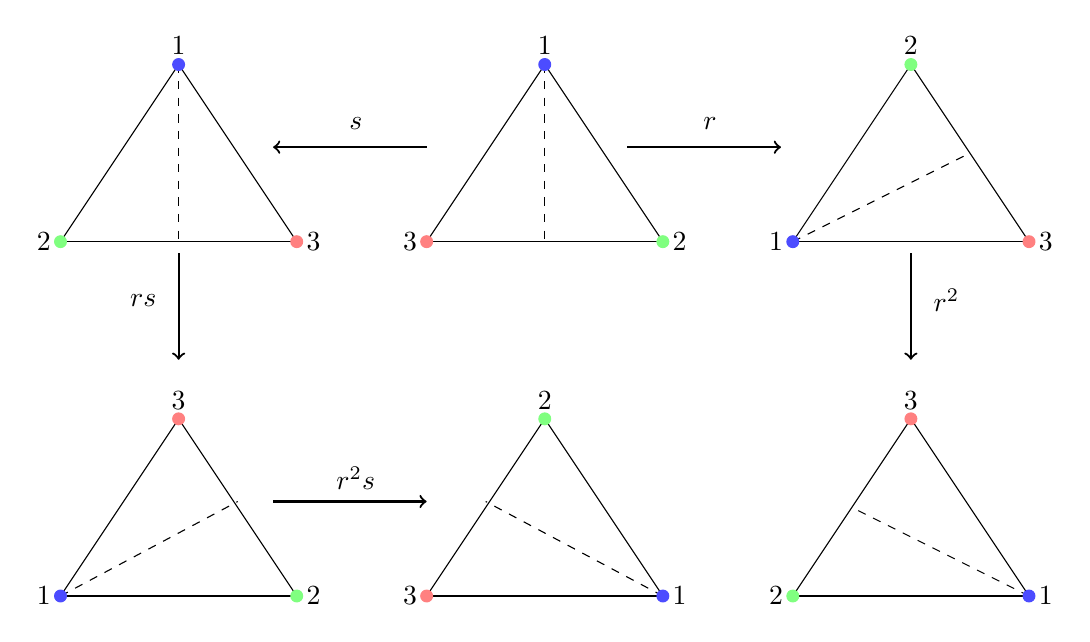
\begin{tikzpicture}[black, scale = 1.5]
            %left triangle
            \draw (-4.1,0) -- (-3.1,1.5) node[above] {$1$};
            \draw (-3.1,1.5) -- (-2.1,0) node[right] {$3$};
            \draw (-2.1, 0) -- (-4.1, 0) node[left] {$2$};
            \draw[dashed] (-3.1, 1.5) -- (-3.1,0);
    
            \filldraw[green!50] (-4.1, 0) circle(0.5mm);
            \filldraw[blue!70] (-3.1, 1.5) circle (0.5mm);
            \filldraw[red!50] (-2.1, 0) circle (0.5mm);
    
            %s arrow
            \draw[thick, <-] (-2.3,0.8) to (-1,0.8) node at (-1.6,
            1.0) {$s$};

            %middle left triangle
            \draw (-4.1,-3) -- (-3.1,-1.5) node[above] {$3$};
            \draw (-3.1,-1.5) -- (-2.1,-3) node[right] {$2$};
            \draw (-2.1, -3) -- (-4.1, -3) node[left] {$1$};
            \draw[dashed] (-4.1, -3) -- (-2.6,-2.2);
    
            \filldraw[blue!70] (-4.1, -3) circle(0.5mm);
            \filldraw[red!50] (-3.1, -1.5) circle (0.5mm);
            \filldraw[green!50] (-2.1, -3) circle (0.5mm);
    
            %sr arrow
            \draw[thick, ->] (-3.1, -0.1) to (-3.1, -1) node at (-3.4,
            -0.5) {$rs$};

                    %middle center triangle.
                    \draw (-1,-3) -- (0,-1.5) node[above] {$2$};
                    \draw (0,-1.5) -- (1,-3) node[right] {$1$};
                    \draw (1, -3) -- (-1, -3) node[left] {$3$};
                    \draw[dashed] (1, -3) -- (-0.5,-2.2);
            
                    \filldraw[red!50] (-1, -3) circle(0.5mm);
                    \filldraw[green!50] (0, -1.5) circle (0.5mm);
                    \filldraw[blue!70] (1, -3) circle (0.5mm);
                    
                    %r arrow
                    \draw[thick, ->] (-2.3,-2.2) to (-1,-2.2) node at (-1.6,
                    -2) {$r^2s$};
    
            %center triangle
            \draw (-1,0) -- (0,1.5) node[above] {$1$};
            \draw (0,1.5) -- (1,0) node[right] {$2$};
            \draw (1, 0) -- (-1, 0) node[left] {$3$};
            \draw[dashed] (0, 1.5) -- (0,0);
    
            \filldraw[red!50] (-1, 0) circle(0.5mm);
            \filldraw[blue!70] (0, 1.5) circle (0.5mm);
            \filldraw[green!50] (1, 0) circle (0.5mm);
            
            %r arrow
            \draw[thick, ->] (0.7,0.8) to (2,0.8) node at (1.4,
            1.0) {$r$};
            
            %right triangle
            \draw (2.1,0) -- (3.1,1.5) node[above] {$2$};
            \draw (3.1,1.5) -- (4.1,0) node[right] {$3$};
            \draw (4.1, 0) -- (2.1, 0) node[left] {$1$};
            \draw[dashed] (2.1,0) -- (3.6, 0.75);
    
            \filldraw[blue!70] (2.1, 0) circle(0.5mm);
            \filldraw[green!50] (3.1, 1.5) circle (0.5mm);
            \filldraw[red!50] (4.1, 0) circle (0.5mm);

            %r^2 arrow
            \draw[thick, ->] (3.1,-0.1) to (3.1,-1) node at (3.4,
            -0.5) {$r^2$};

            %middle right triangle
            \draw (2.1,-3) -- (3.1,-1.5) node[above] {$3$};
            \draw (3.1,-1.5) -- (4.1,-3) node[right] {$1$};
            \draw (4.1, -3) -- (2.1, -3) node[left] {$2$};
            \draw[dashed] (4.1,-3) -- (2.6, -2.25);
    
            \filldraw[green!50] (2.1, -3) circle(0.5mm);
            \filldraw[red!50] (3.1, -1.5) circle (0.5mm);
            \filldraw[blue!70] (4.1, -3) circle (0.5mm);


        \end{tikzpicture}
    \end{figure}
\begin{thm}
    Let $(G, \cdot)$ be a group. Then the following hold:
    \begin{itemize}
        \item[1.] The identity $e \in G$ is unique
        \item[2.] The inverse $g^{-1} \in G$ is unique for every $g
        \in G$.
        \item[3.] For any $g \in G$, $(g^{-1})^{-1} = g$. 
        \item[4.] Let $g, h \in G$. Then $(g \cdot h)^{-1} = h^{-1} \cdot g^{-1}$.   
        \item[5.] Let $g_1, g_2, \dots, g_n \in G$. The product $g_1
        \cdot g_2 \cdot \vspace{0.01mm} \dots \vspace{0.01mm} \cdot
        g_n$ is independent of its bracketing. 
        \item[6.] Let $g, h \in G$. There always exist $x, y$ such
        that $g \cdot x = h$ and $h \cdot y = g$.
    \end{itemize}
\end{thm}

\begin{prf}
    \begin{description}
        \item[1.] Suppose there exists another identity 
        element $f$, different from $e$, such that
        $g \cdot f = f \cdot g = g$ for all $g \in G$. Then 
        \[
            e = e \cdot f = f
        \]
        so that $e = f$. Therefore, the identity element is unique.

        \item[2.] Suppose $h_1$ and $h_2$ are both inverses of $g \in
        G$. Then by definition, $h_2 \cdot g = e = g \cdot h_2$ and $h_1 \cdot g = e
        = g \cdot h_1$. Therefore, 
        \[
            h_1 = (h_2 \cdot g) \cdot h_1 = \underbrace{h_2 \cdot (g \cdot h_2)}_{\text{by associativity of G}}
            = h_2 \cdot e = h_2.
        \]
        Thus $h_1 = h_2$, so that the inverse of $g$ os unique. 

        \item[3.] Observe that for any $g \in G$,
        \[
            g^{-1}\cdot (g^{-1})^{-1} = e
        \]
        by defintion. Multiplying on the left by $g$ on both sides of
        the equation, we get 
        \begin{align*}
            g \cdot (g^{-1} \cdot (g^{-1})^{-1}) = g \cdot e
            \implies (g \cdot g^{-1}) \cdot (g^{-1})^{-1} = g 
        \end{align*}
        by associativity. Since $g \cdot g^{-1} = e$, this then leads to 
        \begin{align*}
            e \cdot (g^{-1})^{-1} = g \implies (g^{-1})^{-1} = g
        \end{align*}
        as desired.

        \item[4.] Note that $(g \cdot h)^{-1} \cdot (g \cdot h) = e.$
        Therefore,
        \[
            (g \cdot h)^{-1} \cdot (g \cdot h) = e \implies (g \cdot h)^{-1} \cdot g = h^{-1}
            \implies (g \cdot h)^{-1} = h^{-1} \cdot g^{-1}
        \] 
        by first multiplying on the right by $g^{-1}$ and then by
        $h^{-1}$, which proves the formula.

        \item[5.] We can demonstrate this by induction. First write
        our proposition as
        \[
            P(n)
            =
            \begin{cases}
            \text{For any } g_1, g_2, \dots, g_n \in G\text{ we have that }\\
             g_1\cdot g_2 \cdots g_n \text{ is independent of its bracketing. }
            \end{cases}
        \] 
        \begin{description}
            \item[Base Case.]
            For the base case $n = 1$, there is nothing to check.
            \item[Inductive Step.]
            Now suppose that $P(n)$ is true for all positive integers
            $n \le n_0$. Then let $g_1, g_2, \dots g_{n+1}
            \in G$ and consider 
            \[
                g_1\cdot g_2 \cdots \cdot g_{n+1}.
            \]
            Observe that we clearly have that 
            \[
                g_1\cdot g_2 \cdots \cdot g_{n+1}. = (g_1\cdot g_2 \cdots \cdot g_{i})\cdot(g_{i+1} \cdots \cdot g_{n+1}).
            \]
            for all $1 \le i le n + 1$. Hence we can apply the
            inductive hyptohesis to each of the subproducts $(g_1\cdot
            g_2 \cdots \cdot g_{i})$ and $(g_{i+1} \cdots \cdot
            g_{n+1})$ generated
            in each case. Since this exhausts all possible
            subproducts, and the values do not change by our inductive
            hypothesis, we see that $P(n + 1)$ is true. Hence $P(n)$
            holds for all $n \in \mathbb{N}$. 
        \end{description}

        \item[6.] Observe that if we have the equation $g \cdot x =
        h$, then we can multiply both sides on the right by $g^{-1}$
        to observe that 
        \[
            (g^{-1} \cdot g) \cdot x = g^{-1} \cdot h \implies x = g^{-1} \cdot h.
        \]
        Since $x$ is the product of elements of $G$ (namely, $g^{-1}
        \cdot h$) and because $G$ is closed under $\cdot$, we have
        that $x \in G$. Thus a solution exists in $G$. The proof for
        the existence of $y \in G$ such that $h \cdot y = g$ is
        exactly the same.
    \end{description}
\end{prf}

In our study of group theory, many of the groups we'll deal with will
actually turn out to be finite. We'll also be interested in breaking
down the structures of finite groups (a lot of things can happen). 
A couple things should be noted about finite groups.

{\color{MidnightBlue}
Consider $g \in G$, where $G$ is a \textbf{finite group}. Since $G$ must be
closed under its product, we note that $g^2 \in G$, $g^3 \in G$, and so
on. That is, all powers of $g$ must be in $G$. But since $G$ is
\textit{finite}, there must exist some $m \in
\mathbb{N}$ such that $g^m = e$. If not, you could keep raising the
power of $g$, and keep getting new elements. Since you'd never come
back to $e$, you could then generate an infinite set
$\{g, g^2, g^3, g^4, \dots\}$ entirely contained in $G$. But this
would imply $G$ is infinite, which it isn't.}

\noindent
\begin{definition}
    Let $G$ be a group. The \textbf{order of an element} $g \in G$ is
    the smallest integer $n$ such that $g^n = e$. 

    In addition, if $G$ is a finite group, then we can also talk about
    the \textbf{order of a group} $|G|$, which we define as the number of
    elements within the group.
    
    The order is denoted
    as $|g|$; thus we'd say that $|g| = n$ if $g$ has order $n$. If
    $G$ is infinite, it may be possible that $|g| = \infty$. On the
    topic of order, we define that $g^0 = e$.
\end{definition}
\subsection*{Subgroups.}
    \begin{definition}
        Let $G$ be a group, and consider a subset $H$ of $G$. We define
    $H$ to be \textbf{subgroup} of $G$ if $H$ is also a group.
    \end{definition}
    
    {\color{blue}The definition is exactly what it sounds like: $H$ is a subgroup
    if $H \subset G$ and $H$ is a group. You might note that the
    definition is clear, but determining if a set is a subgroup of $G$
    sounds like a lot of work. Fortunately there's the subgroup test.
    }

    \begin{thm}\label{subgroup_test}
        Let $H$ be nonempty and suppose $H \subset G$. Then $H$ is a
        subgroup if and only if for all $x, y \in H$, $xy^{-1} \in H$.
    \end{thm}

    
    

    \noindent \textbf{If $\mathbf{H}$ is a subgroup, we usually write $\mathbf{H \le G}$ if we
    are trying to be concise.}

    \begin{prf}

        ($\implies$) Suppose $H \le G$. Then since $H$ is a group,
        for any $x, y \in H$, $xy^{-1} \in H$ since it is closed under
        multiplication of its elements. This proves the forward
        direction.
        \\
        
        ($\impliedby$) Suppose $H$ is nonempty and $H \subset G$ such
        that for all $x, y \in H$, $xy^{-1} \in H$. We just need to
        prove $H$ is a group. We already know group multiplication is
        an associative, binary operation on $G$, so it is still
        associative on elements of $H$. Thus we only need to prove
        closedness, existence of identity and inverses.
        
        By the definition of $H$, for all $x, y \in H$, $xy^{-1} \in
        H$. 
        \begin{description}
            \item[Identity.] Let $x \in H$. Then clearly $xx^{-1} = e \in H$. Thus $H$
            has the identity.
            \item[Inverses.] Since $x, e \in H$, we see that $ex^{-1} =
            x^{-1} \in H$. Thus for all $x \in H$, $x^{-1} \in H$.
            \item[Closedness.] Now let $y \in H$; hence, $y^{-1} \in H$, as just proven. Then
            $x(y^{-1})^{-1} = xy\in H$, so that $H$ is closed under
            multiplication of its elements.
        \end{description} 
        Therefore $H$ is (1) a group
        and (2) a subset of $G$ so that $H \le G$, as desired.
    \end{prf}

    It turns out the intersection of two subgroups is still a
    subgroup. In fact, the arbitrary intersection of subgroups always
    produces a subgroup. 
    \begin{thm}
        Let $G$ be a group and $\{H_\alpha\}_{\alpha \in \lambda}$ be
        a family of subgroups of $G$. Then the set $H =
        \bigcap_{\alpha \in \lambda} H_\alpha$ is a subgroup of $G$.
    \end{thm}

    \begin{prf}
        First, observe that 
        \[
            H = \bigcap_{\alpha \in \lambda} H_\alpha
        \]
        is nonempty. This is because each $H_\alpha \le G$ and thus
       the identity of $G$ is contained in each $H_\alpha$ for all
       $\alpha \in \lambda$. So the identity is in $H$ as well.

       Thus let $x, y \in H$. Then $x, y \in H_\alpha$ for all $\alpha
       \in \lambda$. Since each $H_\alpha$ is a group, $y^{-1}$ exists
       and is contained in each $H_\alpha$. Hence, $xy^{-1} \in
       H_\alpha$ for all $\alpha \in \lambda$, so we have that
       $xy^{-1} \in H$. Therefore, we see by the subgroup text that $H
       \le G$. 
    \end{prf}
    With the basic properties of a group introduced, we now introduce
    two more group definitions. 

    \begin{definition}
        Let $G$ be a group and $S \subset G$. The \textbf{centralizer}
        of $S$ in $G$ is defined to be the set $C_G(S)$
        \[
            \textcolor{NavyBlue}{C_G(S)} = \{g \in G \mid gs = sg \text{ for all } s \in S\}.
        \]
    \end{definition}
    In the case where $G$ is abelian, we $C_G(S) = G$ for any nonempty
    subset $S$ of $G$. This definition is close to the \textbf{center
    of a group}, which is as follows.

    \begin{definition}
        Let $G$ be a group. Then the \textbf{center of a group} $G$ is
        defined as 
        \[
            Z(G) = \{z \in G \mid zg = gz \text{ for all } g \in G\}.
        \]
    \end{definition}

    In this case, we note that $C_G(G) = Z(G)$ and if $G$ is abelian
    $Z(G) = G$. Finally, we introduce the definition of the
    normalizer.
    
    \begin{definition}
        Let $G$ be a group and $S \subset G$. The \textbf{normalizer}
        of $S$ in $G$ is defined as 
        \[
            \textcolor{purple}{N_G(S)} = \{g \in G \mid gS = Sg\}
        \]
    \end{definition}
    
    The centralizer and the normalizer are closely related
    definitions. However, these two concepts highlight the important
    distinction one must understand between term-by-term equality and
    set equality. \textcolor{NavyBlue}{Firstly, we can think of $C_G(S)$ as all $g \in G$
    which commutes with each and every single element of $S$.} 
    \textcolor{purple}{On the
    other hand, if $g \in N_G(S)$, it is not necessarily true that $gs
    = sg$ for all $s \in S$. The only requirement is that $gS$
    creates the same set as $Sg$. Of course, one way to do this is
    if $gs = sg$ for all $s \in G$. In that case, $gS = Sg$. But there
    are other ways to do this, so this definition is more versatile
    than $C_G(S)$.}

    One interesting fact is that $C_G(S)$ and $N_G(S)$ are subgroups
    of $G$ for any $S \subset G$. 

    \begin{thm}
        Let $G$ be a group and $S \subset G$. Then $C_G(S)$ and
        $N_G(S)$ are both subgroups of $G$.
    \end{thm}
    \textcolor{blue}{Note: if we let $S = G$, we see that $C_G(S) =
    Z(G)$. 
    Therefore, an immediate corollay of this theorem is that $Z(G)$ is
    also a subgroup of $G$!}

    \begin{prf}
        Let $G$ be a group and $S \subset G$. To show that $C_G(S) \le
        G$, we can use the subgroup test. 
        \begin{description}
            \item[Nonempty.] First we have to show the set is
            nonempty. But note that for any $S$, $e \in C_G(S)$ 
            since $gs = sg$ for any $s \in S$.

            \item[Inverses.] We now show that if $x, y \in C_G(S)$
            then so is $xy^{-1}$. We know that for all $s \in S$, $xs
            = sx$ and $ys = sy$. Therefore $s = y^{-1}sy$ and $s =
            ysy^{-1}$ by solving for $s$ in the last equation.
            Plugging this into the first equation with $x$, we get 
            \[
                xs = sx \implies x(y^{-1}sy) = (ysy^{-1})x 
                \implies xy^{-1}sy = ysy^{-1}x.
            \]
            Multiplying both sides on the right by $y^{-1}$ leads to 
            \[
                xy^{-1}s = ysy^{-1}xy^{-1} 
                \implies xy^{-1}s = syy^{-1}xy^{-1}
                \implies xy^{-1}s = sxy^{-1}
            \]
            where in the second step we used the fact that $ys = sy$.
            Thus $xy^{-1} \in C_G(S)$, so by subgroup test we have
            that $C_G(S) \le G$. 
        \end{description}

        The proof for $N_G(S)$ is the exact same; simply replace $s$
        with $S$.
    \end{prf}

    \newpage
    \section{Permutation Groups.}
    One of the most important and well-known types of groups are the
    permutation groups, which we introduce formally as follows. 

    Consider a finite set of elements $X = \{1, 2, \dots, n\}$. We
    define a 
    \textbf{permutation} to be a reordering of the elements of $X$.
    More formally, a \textbf{permutation} is a bijective mapping
    $\sigma: X \to X$, similar to one that follows. 

    How can we represent this information? We generally don't use sets
    to represent permutations, since sets 
    don't care about order. That is, $\{1, 2, 3\} = \{3,2,1\}$, etc.  

    Thus for a set $\{1, 2, \dots, n\}$, we can represent a
    permutation $\sigma$ of the set of elements as follows:
    \[
       \sigma =  
       \begin{pmatrix}
            1 & 2 & \cdots & n\\
            \sigma(1) & \sigma(2) & \cdots & \sigma(n)
         \end{pmatrix}
    \]
    where we read this as $1$ is assigned to $\sigma(1)$, 2 is
    assigned to $\sigma(2)$. For example, a permutation that just
    shifts the elements down the line is 
    \[
        \sigma = 
        \begin{pmatrix}
            1 & 2 & \cdots & n\\
            2 & 3 & \cdots & 1
         \end{pmatrix}.
    \]
    That is, $\sigma$ sends 1 to 2, 2 to 3 and eventually $n$ to 1. 
    Here we'll denote the set of all permutations of the set $\{1, 2,
    \dots, n\}$, or more generally a set of $n$ objects (since we can
    always enumerate objects with natural numbers) as $S_n$.
    
    \textcolor{NavyBlue}{What is interesting about this is that if we define
    "multiplication" of elements of $S_n$ to be function composition,
    then the 
     \textbf{set of permutations
    of $X$ form a group} which we show as follows.}
    
    Let $X = \{1, 2, \dots, n\}$. 
    \begin{description}
        \item[Closed.]
        For any $\sigma_1, \sigma_2 \in S_n$, we see that $\sigma_2
        \circ \sigma_1$ is (1) a composition of bijective functions
        and therefore is bijective and (2) a permutation of $X$. One
        way to think about the composition is that $\sigma_1$
        rearranges $X$, and
        $\sigma_2$ rearranges $X$ again. Thus $\sigma_2 \circ \sigma_1
        \in S_n$. 

        \item[Associativity.]
        Associativity is obvious since function composition is
        associative. 

        \item[Identity.]
        Observe that the permutation $\sigma_e: X \to X$ for which 
        $\sigma_e(i) = i$ is technically a permutation of $X$.
        Therefore $\sigma_e$ acts as the identity element in $S_n$. 

        \item[Inverse.]
        Consider a permutation $\sigma \in S_n$. Define $\sigma^{-1}$
        to be the function where if $\sigma(i) = j$, then
        $\sigma^{-1}(j) = i$. Then by construction, (1) $\sigma^{-1}$ is a permutation
        of $X$ and (2) $\sigma \circ \sigma^{-1} = \sigma^{-1} \circ
        \sigma = \sigma_e$. Thus $S_n$ contains inverses and
        composition of the inverses returns $\sigma_e$, the identity.
    \end{description}

    \begin{proposition}
        For all $n \ge 1$, $|S_n| = n!$ 
    \end{proposition}

    \begin{prf}
        This is counting the number of ways to rearrange a set of size
        $n$, which we know from combinatorics to simply be $n!$
    \end{prf}

    Now that we know that $S_n$ is a group, we'll study the properties
    of this group. 

    Recall earlier our notation for representing a permutation $\sigma
    \in S_n$:
    \[
       \sigma =  
       \begin{pmatrix}
            1 & 2 & \cdots & n\\
            \sigma(1) & \sigma(2) & \cdots & \sigma(n)
         \end{pmatrix}
    \]
    This notation sucks, since it includes more information than we
    actually need to. For instance, the top row is always going to be
    the same. 
    
    A better way to write this is through
    \textit{cycle decomposition}, which we will soon define.

    \begin{definition}
        Let $\sigma \in S_n$ and suppose $X = \{1, 2, \dots, n\}.$ 
        Suppose that there exists a subset $\{n_1, n_2, \dots, n_k\}$
        of $X$
        such that 
        \begin{align*}
            \sigma(n_1) = n_2, \sigma(n_2) = n_3, \dots, \sigma(n_k) = n_1.
        \end{align*}
        Then $\{n_1, n_2, \dots, n_k\}$ is called a 
        \textbf{cycle},
        and we denote this cycle as 
        \[
            \sigma = \begin{pmatrix}
                n_1 & n_2 & \cdots & n_k
            \end{pmatrix}.
        \]
        We then read this as "$n_1 \to n_2$, $n_2 \to n_3, \dots, n_k
        \to n_1$". 

        \textcolor{Blue}{\textbf{Why do we care about cycles?}} 
        \\
        Well,
        consider an arbitrary cycle $            \sigma = \begin{pmatrix}
            n_1 & n_2 & \cdots & n_k
        \end{pmatrix}.$ Then again, $\sigma(n_1) = n_2, \sigma(n_2) =
        n_3, \dots, \sigma(n_k) = n_1.$ However, what this is really
        saying is that 
        \[
            \sigma(n_1) = n_2, \sigma^2(n_1) = n_3, \dots, \sigma^{{k-1}}(n_1) = n_k, \sigma^k(n_1) = n_1.
        \]
        However, also take a note to observe that 
        \[
            \sigma(n_2) = n_3, \sigma^2(n_2) = n_4, \dots, \sigma^{{k-1}}(n_2) = n_1, \sigma^k(n_2) = n_2.
        \]
        More generally, we see that \textcolor{blue}{the element $\sigma \in S_n$ has
        order $n_k$}, which is why the cycle length is $k$. 

        \textcolor{Blue}{\textbf{We care about cycles}} since, given the fact that $S_n$
        is always a finite group, each of its elements will have
        finite order. Thus, in some way, we can always represent the
        elements of $S_n$ in this form.
        \\
        \\
        \textbf{More definitions.}
        \\
        If $            \begin{pmatrix}
            n_1 & n_2 & \cdots & n_k
        \end{pmatrix}$ and $            \begin{pmatrix}
            n'_1 & n'_2 & \cdots & n'_k
        \end{pmatrix}$ 
        share no elements in common, i.e., 
        \[
            \{n_1, n_2, \dots, n_k\} \cap \{n_1', n_2', 
            \dots, n_k'\} = \varnothing
        \]

        then the cycles are defined as
        \textbf{disjoint cycles}.
        \\

        Note that if $\sigma(i) = i$ for some $i \in X$, then this is
        technically a cycle and we represent the cycle as $            \begin{pmatrix}
            i
        \end{pmatrix}.$ In this case, we say that $\sigma$ \textbf{fixes} $i$.
        \\

        For example, suppose we have a permutation $\sigma \in S_5$
        where $\sigma(1) = 2, \sigma(2) = 4, \sigma(4) = 2$. Then we
        have a cycle of length 4 and we denote this as 
        \[
            \begin{pmatrix}
                1 & 2 & 4
            \end{pmatrix}.
        \]
        Since $\sigma \in S_5$, suppose further
        that $\sigma(3) = 5$ and $\sigma(5) = 3$. Then we see that we
        have another cycle, disjoint with the previous cycle, and we write this one as
        \[
            \begin{pmatrix}
                3 & 5
            \end{pmatrix}.
        \]
        To write the entire permutation, we then can then express
        $\sigma$ as 
        \[
            \sigma =  \begin{pmatrix}
                1 & 2 & 4
            \end{pmatrix}
            \begin{pmatrix}
                3 & 5
            \end{pmatrix}
        \]
        which gives us all the information we need to know on how
        $\sigma$ rearranges the elements of $X$. Such a representation
        of a permutation is called a \textbf{disjoint cycle decomposition}. 
        It will turn out that
        we can actually express \textit{every} permutation $\sigma \in
        S_n$ in a product of disjoint cycles.
    \end{definition}
    \textbf{Remark.}
    In general, 1-cycles are omitted in the representation of a
    disjoint cycle decomposition. Thus if we have a permutation
    $\sigma \in S_3$ such that $\sigma(1) = 2$, $\sigma(2) = 1$ and
    $\sigma(3) = 3$, then we would write this as 
    \[
        \sigma = \begin{pmatrix}
            1 & 2
        \end{pmatrix}.
    \]
    Such a statement leads us to conclude that $\sigma(3) = 3$. And if
    $\sigma \in S_5$, we would furthermore conclude that not only $\sigma(3) =
    3$, but also $\sigma(4) = 4$ and $\sigma(5) = 5$.
    \\
    \\
    \textbf{Nonuniqueness.}
    One thing to note is that cycles are not unique. For example, we
    could have written the cycle $\textcolor{ForestGreen}{\begin{pmatrix}
        1 & 2 & 4
    \end{pmatrix}} $ as $\textcolor{OrangeRed}{\begin{pmatrix}
        2 & 4 & 1
    \end{pmatrix}}$ or $\textcolor{Cyan}{\begin{pmatrix}
        4 & 1 & 2
    \end{pmatrix}}$, since the other expressions still capture the fact
    that 1 is sent to 2, 2 is sent to 4, and 4 is sent to 1. 
    \begin{center}
        \begin{tikzcd}
            & 4 \arrow[dr, color = Cyan] & \\
            2 \arrow[ur, color = OrangeRed] & & 1\arrow[ll, color = ForestGreen]
            \end{tikzcd}.
    \end{center}
    Note that the colors correspond to where the cycle starts. Clearly
    in the diagram, there are three ways to start the cycle, and hence
    why there are three nonunique representations for the cycle. 
    \\
    More
    generally, for any cycle $            \begin{pmatrix}
        i_1 & i_2 & \cdots & i_n
    \end{pmatrix}$ we have that 
    \[
        \begin{pmatrix}
            i_1 & i_2 & \cdots & i_n
        \end{pmatrix}
        = \begin{pmatrix}
            i_2 & i_3 & \cdots & i_n & i_1
        \end{pmatrix}
        = 
        \cdots 
        = 
        \begin{pmatrix}
            i_n & i_1 & \cdots & i_{n-1}
        \end{pmatrix}.
    \]





    \newpage
    \section{Homomorphism and Isomorphisms.} 
    {\color{BlueViolet}As with all mathematical objects, now that we have a well defined
    abstract concept (i.e., a group) we'll now be interested
    attempting to understand \textit{mappings} between different
    groups. Mappings of abstract concepts simply helps mathematicians
    get a better sense of what they're dealing with, and most often
    provides new insight into understand their objects. 
    
    The most important utility of the following definition is that it
    not only leads one to have a better understanding of groups, but it
    also helps us understand when two groups are equivalent. For
    example, $D_3$ and $S_3$ equivalent, since one could view $D_3$
    as simply all the permutations of 1, 2, and 3, if we assigned these
    numbers to the vertices of a triangle.
    }

    \begin{definition}
        Let $(G, \cdot)$ and $(G', *)$ be groups. A
        \textbf{homomorphism} is a mapping $\phi: G \to G'$ such that,
       for all $a, b \in G$, 
        \[
            \phi(a \cdot b) = \phi(a) * \phi(b).
        \]
        {\color{red}Again, here $*$ is the group operation of $G'$.}

    \end{definition}

    \textbf{Example.} Consider the two groups $GL_n(\mathbb{R})$ and
    $\mathbb{R}\setminus\{0\}$. If we define $\phi$ such that, for $A \in
    GL_n(\mathbb{R})$ 
    \[
        \phi(A) = \det(A)
    \]
    then $\phi$ defines a homomorphism. 
    
    Recall that for for any $n
    \times n$ matrices $A, B$ that $\det(AB) = \det(A)\det(B)$.
    Therefore 
    \[
        \phi(AB) = \det(AB) = \det(A)\det(B) = \phi(A)\phi(B).
    \]
    Since $\phi(AB) = \phi(A)\phi(B)$, we see that $\phi$ satisfies
    the condition to be a homomorphism.

    \begin{proposition}
        Let $\phi: G \to G'$ be a homomorphism. Then all of the
        following hold.
        \begin{itemize}
            \item[1.] If $e_G$ is the identity of $G$ and $e_{G'}$ is
            the identity of $G'$, then $\phi(e_G) = e_{G'}$.

            \item[2.] For all $g \in G$, $\phi(g^{-1}) =
            \phi(g)^{-1}$. 

            \item[3.] For $g_1, g_2, \dots, g_n \in G$, then $\phi(g_1
            \cdot g_2 \cdot \dots \cdot g_n) =
            \phi(g_1)\phi(g_2)\cdots\phi(g_n)$. Consequently, if $g = g_1 =
            g_2 = \cdots = g_n$, then $\phi(g^n) = \phi(g)^{n}$.
        \end{itemize}
    \end{proposition}

    \begin{prf}
        Let $g \in G$, and suppose $\phi: G \to G'$ is a
        homomorphism. 
        
        \begin{itemize}
            \item[1.] Since $e_G = e_G \cdot e_G$, we have that 
            \[
                \phi(e_G) = \phi(e_G \cdot e_G) = \phi(e_G)\phi(e_G).
            \] 
            We also know that $\phi(e_G) \in G'$, and becuase $G'$ is a group,
            there exists an inverse $\phi(e_G)^{-1} \in G$ of
            $\phi(e_G)$. Multiplying this on the left (or right)
            yields
            \[
                e_{G'} = \phi(e_G)  
            \]
            as desired.
            \item[2.] Since $gg^{-1} = e_G$, and by (1.) we know that
            $\phi(e_G) = e_{G'}$. Hence 
            \[
                \phi(e_G) = e_{G'} \implies \phi(gg^{-1}) = e_{G'} 
                \implies \phi(g)\phi(g^{-1}) = e_{G'}.
            \]
            Again, $\phi(g) \in G'$, and since $G'$ is a group there
            exist an inverse $\phi(g)^{-1} \in G$ of $\phi(g)$.
            Multiplying on the left by this inverse, we get 
            \[
                \phi(g)\phi(g^{-1}) = e_{G'} \implies \phi(g^{-1}) = \phi(g)^{-1}
            \]
            as desired.

            \item[3.] This is just repeated application of the
            homomorphism property. 
            For $g_1, g_2, \dots g_n \in G$, $g_1 \cdot
            g_2 \cdot \hspace{0.01mm} \dots \hspace{0.01mm} \cdot g_n = g_1 \cdot (g')$ 
            where $g' = g_2
            \cdot g_3 \cdot \hspace{0.01mm} \dots \hspace{0.01mm} \cdot g_n$. Applying the
            homomorphism property, 
            \[
                \phi(g_1 \cdot g_2 \cdot \hspace{0.01mm} \dots \hspace{0.01mm} \cdot g_n) = \phi(g_1 \cdot g') = \phi(g_1) \phi(g').
            \]
            Repeatedly applying the same idea, starting again with the
            product $g_2 \cdot g_3 \cdot \hspace{0.01mm} \dots
            \hspace{0.01mm} \cdot g_n$ yields the result. The fact
            that $\phi(g^n) = \phi(g)^n$ is follows immediately.
        \end{itemize}
    \end{prf}
    {\color{Plum} 
    If $\phi$ is a bijective homomorphism (i.e., one-to-one and
    onto) then we say that $\phi$ is an \textbf{isomorphism}.
    Furthermore, if there exists an isomorphism between two spaces
    $G$ and $G'$, then we say these spaces are \textbf{isomorphic}
    and that $G \cong G'$. As we'll soon see, isomorphisms gives
    us really nice results (hence the special terminology and
    notation). In addition, it can sometimes be difficult to tell when
    two groups $G$ and $G'$ are the same or different. Isomorphisms
    can help determine when there \textit{isn't} such an equivalence.

    As we'll see, the concept of an isomorphism is very powerful.
    However, proving it may not be that simple, and in ceratin cases
    the following theorem will be very useful.
    }

    \begin{thm}
        Let $G$ and $H$ be groups. The homomorphism $\phi: G \to H$ is an
        isomorphism if and only if there exists a homomorphism $\psi:
        H \to G$ such that $\psi \circ \phi$ is the identity map on
        $G$ and $\phi \circ \psi$ is the identity map on
        $H$.
    \end{thm}

    \begin{prf}
        ($\implies$) Suppose $\phi: G \to H$ is an isomorphism. Since
        $\phi$ is bijective, define the inverse map $\phi^{-1}: H \to
        G$ such that if $\phi(g) = g'$ then $\phi^{-1}(g') = g$. 

        Note that this is a well defined map due to the surjectivity
        and injectivity of $\phi$. To show it is a homomorphism, we
        need to demonstrate that $\phi^{-1}(h_1\cdot h_2) =
        \phi^{-1}(h_1)\phi^{-1}(h_2)$. Thus 
        observe that for $h_1, h_2 \in H$ there exist $g_1, g_2 \in G$
        such that $\phi(g_1) = h_1$ and $\phi(g_2) = h_2$. Therefore
        \[
            \phi(g_1 \cdot g_2) = h_1 \cdot h_2 \implies \phi^{-1}(h_1 \cdot h_2) = g_1\cdot g_2
            = \phi^{-1}(h_1)\cdot\phi^{-1}(h_2).
        \]
        Thus $\phi^{-1}$ is a homomorphism.

        Now observe that for all $g \in G$ we have that $\phi^{-1}
        \circ \phi(g) = g$ and for all $h \in H$, $\phi \circ \phi^{-1}(h) =
        h.$ Thus $\phi^{-1} \circ \phi$ is the identity on $G$ while
        $\phi \circ \phi^{-1}$ is the identity on $H$, which proves
        this direction.

        ($\impliedby$) Now suppose $\phi: G \to H$ is a homomorphism
        and that there exists a homomorphism
        $\psi: H \to G$ such that $\psi \circ \phi$ is the identity
        map on $G$ and $\phi \circ \psi$ is the identity map in $H$.
        In other words, $\psi$ and $\phi$ are inverses of each other. 
        Thus $\phi$ is a bijection function from $G \to H$, which
        implies that $\phi$ is an isomorphism. 
    \end{prf}
    
    We also introduce the following criteria which is frequently used
    to evaluate if a homomorphism is one-to-one and/or onto. 
    
    \begin{thm}\label{theorem_isomorph}
        Let $\phi: G \to G'$ be a homomorphism.
        Then 
        \begin{itemize}
            \item[1.] $\phi$ is one-to-one if and only if
            $\mbox{ker}(\phi)$ is trivial. That is, $\mbox{ker}(\phi) = \{e_G\}$, where $e_G$ is
            the identity of $G$.

            \item[2.] $\phi$ is onto if and only if $\mbox{im}(\phi) = G'$. 
        \end{itemize}
        Therefore, $\phi$ is an \textbf{isomorphism} if and only if
        (1) and (2) hold.
    \end{thm}

    \begin{prf}
        \begin{itemize}
            \item[1.] Suppose $\phi$ is one-to-one. By proposition
            1.1.1, we know that $\phi(e_G) = e_{G'}$. But since $\phi$
            is injective we know $e_G$ is the only element in $G$
            which is mapped to $e_{G'}$. Therefore $\mbox{ker}(\phi) =
            \{e_G\}$.

            Now suppose $\mbox{ker}(\phi) = \{e_G\}$. To show $\phi$
            is one-to-one, consider
            $g, h \in G$ such that
            \[
                \phi(g) = \phi(h).
            \]
            Multiplying both sides by $\phi(h)^{-1}$ we get 
            \[
                \phi(g)\phi(h)^{-1} = e_{G'}.
            \]
            By proposition 1.1.2, we know that $\phi(h)^{-1} =
            \phi(h^{-1})$. Since $\phi$ is a homomorphism, we can then
           combine the terms to get 
           \[
                \phi(gh^{-1}) = e_{G'}.
           \] 
           Since $\mbox{ker}(\phi) = \{e_G\}$, we see that 
           \[
                gh^{-1} = e_G \implies g = h.                
           \]
           Therefore $\phi$ is one to one.
           
           \item[2.] Suppose $\phi$ is onto. Then $\mbox{im}(\phi) = G'$
           is just another way of stating this fact. 
           
           Suppose $\mbox{im}(\phi) = G'$. Then for every element $g'
           \in G'$, there exists $g \in G$ such that $\phi(g) = g'$.
           That is, $\phi$ covers every value in $G'$ so that it is
           onto.
        \end{itemize}
        Thus, we have that a function is isomorphic if and only if it
        is one to one and onto. Hence, it is isomorphic if and only if
        (1) and (2) hold.
    \end{prf}

    We also make two common definitions for special homomorphisms. 
    \begin{definition}
        Let $G$ be a group.
        \begin{itemize}
            \item[1.] If $\phi: G \to G$ is a group homomorphism, then
            we say that $\phi$ is a \textbf{endomorphism}.
            \item[2.] If $\phi$ is a bijective endomorphism (an
            isomophic endomorphism) then we say that $\phi$ is an \textbf{automorphism}.
        \end{itemize} 
    \end{definition}

    \begin{thm}
        The set of all automorphisms of a group $G$, denoted as
        $\text{Aut}(G)$, forms a group with an operation $\circ$ of
        function composition.
    \end{thm}

    \begin{prf}
        We can prove this directly. 
        \begin{description}
            \item[Closure.] Let $\phi$ and $\psi$ be automorphisms.
            Then $\phi \circ \psi$ is (1) a homomorphism from $G \to
            G$ and (2) a bijection (as the composition of bijections
            is a bijetion).

            \item[Associativity.] In general, function composition is
            associative. 

            \item[Identity.] Let $i:G \to G$ be the identity map. The
            (1) $i$ is a group homomorphism and (2) a bijection.
            Therefore $i \in \text{Aut}(G)$ and we can set $i$ as the
            identity of the group. Note that 
            \[
                i \circ \phi = \phi = \phi \circ i   
            \]
            for any $\phi \in \text{Aut}(G)$. 

            \item[Inverse.] Let $\phi \in \text{Aut}(G)$. Construct
            the function $\phi^{-1}$ as follows. If $\phi(g) = g'$ for
            some $g, g' \in G$, then write $\phi^{-1}(g') = g$. Such
            an assignment is well-defined since  $\phi$ is a
            bijection. Hence we see that 
            \[
                \phi \circ \phi^{-1} = i = \phi^{-1} \circ \phi.
            \]
            Finally, observe that $\phi^{-1}$ is (1) a homomorphism
            and (2) a bijection, so we see that $\phi^{-1} \in
            \text{Aut}(G)$. Therefore this forms a group.
        \end{description}
    \end{prf}



    \newpage
    \section{Cyclic Groups.}
    Cyclics groups are a special type of group that are easy to
    recognize as group structures. In a cyclic group, one can always
    pinpoint a single element which can "generate" every other element
    of the group. For example, the subgroup of rotations $\{e, r, r^2,
    \dots, r^{n-1}\}$ in dihedral groups
    is cyclic. In such a subgroup, every element is simply a fininte
    power of $r$. We can then think of this subgroup as
    being generated by a single element, namely $r$.

    It will turn out later that, in every group, there will always be
    a subset of its elements such that the subset generates the whole
    group. Here, we're starting small, by just considering groups
    whose elements can be generated by \textit{one} element.

    \begin{definition}
        A group $G$ is \textbf{cyclic} if there exists an element $g
        \in G$ such that 
        \[
            G = \{g^n \mid n \in \mathbb{N}\}.
        \]
    \end{definition}
    
    A very trivial example of a cyclic group is the integers under
    addition. This is because every element in $(\mathbb{Z}, +)$ can
    be generated by the number 1 (e.g., 3 = 1 + 1 + 1, -2 $= -1 -1$).
    With the definition of cyclic groups at hand, we can introduce
    theorems about cyclic groups.

    \begin{thm}
        Let $G$ be a cyclic group, and suppose $G = \{g^n 
        | n \in \mathbb{N}\}$ for some $g \in G$. Then $|G| = |g|$.
    \end{thm}

    \begin{prf}
        Suppose $|g| = k$ where $k$ is some positive integer. Then 
        since $G = \{g^n | n \in \mathbb{N}\}$, 
        \[
            G = \{e, g, g^2, \dots, g^{k-1}\}.
        \]
        Therefore $|G| = k = |g|$. Now if $|g| = \infty$, then 
        by the same exact reasoning $|G| = \infty$.
    \end{prf}
    A consequence of this theorem is that if $|g| = \infty$, then we
    know that $g^a \ne g^b$ for any $a, b \in \mathbb{N}$ such that $a
    \ne b$. This would imply that $g^{a - b} = 1$, which otherwise 
    imply the group $G$ to have finite order; a contradiction if $|g|
    = \infty$ since this implies $|G| = \infty$.

    \begin{thm}
        Any two cyclic groups of the same order are isomorphic.
    \end{thm}

    \begin{prf}
        Let $G$ and $G'$ be two cyclic groups and suppose $|G| =
        |G'|$. Furthermore suppose that $G = \left< g\right>$ and $G'
        = \left< g' \right>$. Construct the homomorphism $\phi: G \to
        G'$ where 
        \[
            \phi(g^n) = (g')^n
        \]
        for any $n \in \mathbb{N}$. Observe that this is surjective, as
        the groups are of equal order so for any $(g')^n$ there we can
        identify the preimage to be $g^n$. This is also injective,
        since if $g_1' = g_2'$ are both elements in $G'$, then $g_1' =
        g_2' = (g')^n$ for some $n$ which corresponds to one and only
        one element in $G$; namely, $g^n$.
        As the homomorphism we constructed is surjective and
        injective, we have that $\phi$ is an isomorphism so that the
        groups are isomorphic.

        Note we could have also utilized Theorem 1.3 here, by constructing
        the homomorphism $\psi: G' \to G$ where $\psi((g')^n) = g^n$.

    \end{prf}

    We'll now move onto a more useful theorem concerning cyclic groups.

    \begin{thm}
        Let $G$ be a cyclic group. Then every subgroup of $G$ is cyclic.
    \end{thm}

    \begin{prf}
        Let $H$ be a subgroup of $G$.
        Let $m$ be the smallest integer such that $g^m \in H$. Suppose
        towards a contradiction that $H$ is not cyclic. That is, there
        exists an element $h \in H$ such that $h \ne g^{mn}$ for any
        $m \in \mathbb{N}$. 
        
        Since $h \in G$, and $G$ is a cyclic group, it must be \textit{some}
        integer power of $g$. Since $h \ne g^m$ for any $m \in
        \mathbb{N}$, 
        we know that
        there must exist $q, r \in \mathbb{Z}$ such that $h
        = g^{qm + r}$ where $0 < r < m$. 

        Now since $H$ is a group, $h^{-1} = g^{-(qm + r)} \in H$.
        Furthermore, $g^{(q+1)m} \in H$ since $H$ is closed under
        products. By the same reasoning,
        \[
            g^{(q+1)m}g^{-(qm + r)} = g^{m-r}
        \]
        is in $H$. However, this contradicts our assumption that $m$
        is the smallest positive integer such that $g^m \in H$. Thus
        by contradiction $H$ must be cyclic. 
    \end{prf}
    \textbf{Remark.}
    This proof utilizes the important idea that, if you \textit{know} $G$ is
    a group, and $g_1, g_2$ are \textit{any} two elements of $G$, then
    the product $g_1g_2 \in G$. Furthermore, if $g_1, g_2, \dots, g_n
    \in G$, then $g_1^{n_1}g_2^{n_2}\cdots g_k^{n_k} \in G$ for
    literally any powers $n_1, n_2 \dots n_k \in \mathbb{Z}$. 
    
    We used this idea by (1) observing that $g^m \in H$, so that
    $g^{(q+1)m} \in H$ for any $q \in \mathbb{Z}$ and (2) reasoning
    that $g^{(q+1)m}g^{-(qm + r)} \in H$.

    In addition, we'll offer a way to think about subgroups of a
    cyclic group $G$:
    \begin{gather}
        G = \{{\color{blue}e}, g, {\color{blue}g^2}, g^3, {\color{blue}g^4}, g^5, {\color{blue}g^6}, g^7, {\color{blue}g^8}, g^9, g^10, \dots\}\\
          \hspace{0.5cm}= \{{\color{red}e}, g, g^2, {\color{red}g^3}, g^4, g^5, {\color{red}g^6}, g^7, g^8, {\color{red}g^9}, g^{10}, \dots\}\\
          \hspace{0.5cm}= \{{\color{magenta}e}, g, g^2, g^3, {\color{magenta}g^4}, g^5, g^6, g^7, {\color{magenta}g^8}, g^9, g^{10}, \dots\}
    \end{gather}
    In the above representations, the color-highlighted powers of $g$
    form subgroups of $G$. Thus $\{{\color{blue}e}, {\color{blue}g^2},
    {\color{blue}g^4}, {\color{blue}g^6}, \dots\}$, 
    $\{{\color{red}e}, {\color{red}g^3},
    {\color{red}g^6}, {\color{red}g^9}, \dots \}$ and $\{{\color{magenta}e}, {\color{magenta}g^4},
    {\color{magenta}g^8}, \dots\}$ are
    all subgroups of $G$. Of course, this process will eventually terminate if
    $G$ is finite, but we represent the most general case above with
    the $\dots$ terms. In addition, if $G$ is finite one of the
    subgroups may turn out to be just the entire group $G$. 

    To find the exact subgroups of a cyclic group we can use the
    following theorem. 

    \begin{thm}
        Let $G$ be a finite cyclic group of order $n$. For every positive
        integer $d$ such that $d|n$, there is exactly one subgroup of
        order $d$ of $G$. These are all the subgroups of $G$. 
    \end{thm} 

    \begin{prf}
        Let $H$ be a subgroup of $G$ and suppose
        $|H| = m \le n$. We'll first show that $n \mid m$ and then
        show that for every $d \mid n$, there exists a subgroup of
        order $d$.

        By the previous theorem, we
        know that $H$ must be cyclic. Therefore $H = \{h^n \mid n \in
        \mathbb{N}\}$ for some $h \in G$. However, by Theorem 1.4, we
        also know that $|H| = |h|$, so that $h^m = e$. Therefore, 
        \[
            H = \{e, h, h^2, \dots, h^{m-1}\}.
        \] 
        However, if $G = \{e, g, g^2, \dots, g^{n-1}\}$ for some $g \in G$, then $h = g^k$ for some
        positive integer
        $k < n$. Therefore 
        \[
            H = \{g^{jk} \mid j \in \mathbb{N}\}.
        \]
        Since $g^k$ generates $H$, we can apply Theorem 1.4 to
        conclude that $|g^k| = m$. In order for this to be true, there must
        exist some positive integer $j$ such that $g^{jk} = e$.

        On one hand, we already know $m$ is the smallest such integer, as
        we specified $h^m = (g^k)^m = e$. On the other, we also know
        that $|g| = n$; that is, $n$ is the smallest integer such that
        $g^n = e$. Therefore, we have that 
        \[
            n = mk
        \]
        which proves that $m \mid n$. 

        To show that for each $d \mid n$ there exists a subgroup of
        order $d$, simply observe that if $G = \{e, g, g^2, \dots ,
        g^n\}$ then the set $\{e, g^{n/d}, g^{2n/d}, \dots,
        g^{(d-1)n/d}\}$ is a subgroup of order $d$. This completes the
        proof.
    \end{prf}

    \newpage
    \section{Left and Right Cosets, Lagrange's Theorem}

    The result of the previous proof is a special case of a more general
    theorem we'll come across, know as Lagrange's Theorem. The theorem
    states that if $G$ is a finite group and $H$ is a subgroup, then
    $|H| \mid |G|$. That is, the order of $H$ divides $G$. This is a
    remarkable and useful result, aiding proofs as we move on from it.
    But in order to reach Lagrange's Theorem we first discuss the
    extremely important concept of a \textbf{coset} of a group.

    Before defining a coset, we first recall the definition of an
    equivalence relation. 

    \begin{definition}
        An equivalence relation on a set $G$ is a binary relation
        $\sim$ that satisfies the following properties.
        \begin{description}
            \item[Reflexive.] For all $a \in G$, $a \sim a$.
            \item[Symmetric.] If $a \sim b$ then $b \sim a$.
            \item[Transitive.] If $a \sim b$ and $b \sim c$ then $a
            \sim c$. 
        \end{description}
    \end{definition}

    \textcolor{Plum}{Equivalence classes are a useful concept since they tend to break
    up a set of objects $G$ into distinct, disjoint sets $A_i$. More
    specifically, they partition $G$. These sets, $A_i$, are
    known as \textbf{equivalence classes} since their criteria for
    membership requires that $a \in A_i$ if and only if $a \sim a'$ for
    all $a' \in A_i$. 
    This is a general strategy in mathematics: to define equivalence
    classes from \textit{some} equivalence relation to break up a set
    into disjoint partitions. However, we use the
    concept of an equivalence class to partition a group $G$. We use
    the following relation to do this.}
    \\

    \textcolor{blue!90!black!100}{\textbf{The Relation.}}

    Let $G$ be a group and $H$ be a subgroup of $G$. If $a, b \in G$, then the
    relation $\sim$ on $G$ such that $a \sim b$ if and only if $ab^{-1} \in H$
    is an equivalence relation.
  \begin{prf}
    \begin{description}
        \item[Reflexive.] Observe that $a \sim a$, since $aa^{-1} = e
        \in H$.

        \item[Symmetric.] First, if $a \sim b$ then $ab^{-1} \in H$. Since $H$ is a
        group, we know that $(ab^{-1})^{-1} = ba^{-1} \in H$.
        Thus by our definition we see that $b \sim a$, so that our
        relation is also symmetric. 

        \item[Transitive.] Now suppose $a \sim b$ and $b \sim c$ for
        $a, b, c \in G$. Then by definition $ab^{-1} \in H$ and
        $bc^{-1} \in H$. Since $H$ is a group, and it is closed under
        products of its elements. Therefore
        \[
            (ab^{-1})(bc^{-1}) = ab^{-1}bc^{-1} = ac^{-1} \in H.
        \]
        Thus we see that $a \sim c$, which proves that our
        relation is transitive.
    \end{description}
\end{prf}
    As our relation is reflexive, symmetric and transitive, we see
    that it is an equivalence relation. Note however that we could
    have defined our relation as $a \sim b$ if and only if $a^{-1}b
    \in H$; such a relation is equivalent to what we just worked with.

    First we require a quick definition.
    \begin{definition}
        Consider a subgroup $H$ of $G$. For any $a \in G$, we define
        \begin{align*}
            Ha = \{ha \mid \text{ for all }h \in H\}
        \end{align*}
        to be the right coset of $H$. We also define
        \begin{align*} 
            aH = \{ah \mid \text{ for all }h \in H\}. 
        \end{align*}
        to be the left coset of $H$.
        Note that since $H$ is a group, it is closed under products of
        its elements. Therefore for any $h\in H$
        \[
            hH = Hh = H.
        \]
    \end{definition}

    \textcolor{red!80}{Don't confuse the above equality; take special note that 
    equality above is \textit{set equality}, not term by term
    equality. Of course we have no idea if $ha = ah$ where $h \in H$
    for $a \in G$ unless $G$ is abelian or we have other information.}
    \\

    \textcolor{blue!90!black!100}{\textbf{The Big Idea of Cosets.}}

    Now consider the relation introduced earlier, which we 
    proved is in fact an equivalence
    relation. Consider an equivalence class of an element $a \in G$,
    denoted $[a]$. Then we can describe $[a]$ as 
    \begin{gather*}
        [a] = \{g \in G \mid g \sim a \}\\
        \hspace{1.35cm} = \{g \in G \mid ga^{-1} \in H \}\\
        \hspace{4.2cm} = \{g \in G \mid ga^{-1} = h \text{ for some } h \in H \}\\
        \hspace{3.75cm} = \{g \in G \mid g = ha \text{ for some } h \in H \}\\
        \hspace{-1.7cm}= Ha.
    \end{gather*}
    Thus the equivalence classes of the elements of $G$ with respect
    to some subgroup $H$ are simply just the right cosets of $H$. (We
    could have alternatively defined our equivalence relation to be $g
    \sim a$ if and only if $a^{-1}g \in H$, in which case our above
    description of $[a]$ would have resulted in being equal to $aH$. Since both
    formulations are equivalent, we will simply work with the right
    cosets of $H$, namely the sets $Ha$.)

    \begin{figure}[h]
        \centering
        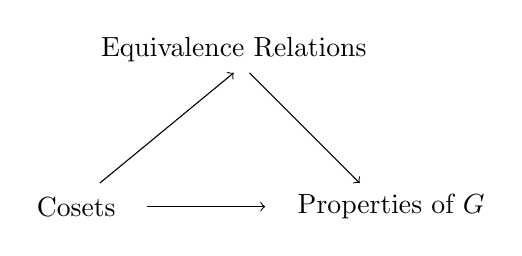
\begin{tikzpicture}
            \node at (0,0) {Cosets};
            \draw[->] (0.3, 0.3) -- (2, 1.7);
            \node at (2, 2) {Equivalence Relations};
            \draw[->] (0.9, 0) -- (2.4, 0);
            \draw[->] (2.2, 1.7) -- (3.6, 0.3);
            \node at (4,0) {Properties of $G$};
        \end{tikzpicture}
    \end{figure}
    Once we understand cosets, we can understand a lot about a group,
    because they're really 
    
    just equivalence classes!
    \vspace{0.8cm}

    \textcolor{NavyBlue!100!black!100}{Since equivalence classes are mathematical objects which partition
    a set, what we have is the following beautiful idea: We can take a
    subgroup $H$ of a set $G$ and partition our group $G$ via the
    right (or left) cosets of $H$. This is because our cosets are
    equivalence classes, and as we said before equivalence classes
    partition sets which they are defined on.}
    \\
    \\
    \textbf{Example}\\
    Consider the group $\ZZ$ and the subgroup $5\ZZ = \{5n \mid n \in \ZZ\}$. 
    We can calculate the cosets of this $\ZZ$ with respect to $5\ZZ$ as 
    \begin{align*}
        5\ZZ + 1 &= \{5n + 1 \mid n \in \ZZ\}\\
        5\ZZ + 2 &= \{5n + 2 \mid n \in \ZZ\}\\
        5\ZZ + 3 &= \{5n + 3 \mid n \in \ZZ\}\\
        5\ZZ + 4 &= \{5n + 4 \mid n \in \ZZ\}\\
        5\ZZ + 5 &= \{5n + 5 \mid n \in \ZZ \} = 5\ZZ
    \end{align*}
    Note that we didn't list any other
    cosets. Well, that's because these are all of the possible
    distinct cosets of $\ZZ$ with respect to $5\ZZ$. For example, the coset $5\ZZ + 37$ is
    equivalent to $5\ZZ + 2$, since 
    \begin{align*}
        5\ZZ + 37 = \{5n + 37 \mid n \in \ZZ\}
        &= \{5n + 5\cdot 7 + 2 \mid n \in \ZZ\}\\
        &=\{5(n+7) + 2 \mid n \in \ZZ\}\\
        &= 5\ZZ + 2.
    \end{align*}
    Thus, any other coset we propose is equivalent to one of the five
    we listed. This is demonstrated in the figure below.

    \begin{figure}[h]
        \centering
        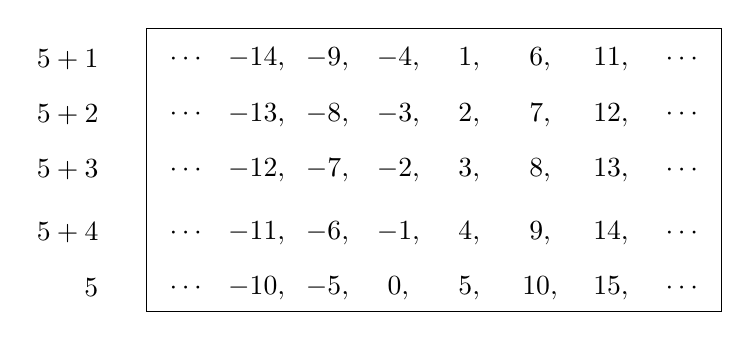
\begin{tikzpicture}
            \node at (-1,3.2) {$5\ZZ + 1$};
            \node at (-1,2.5) {$5\ZZ + 2$};
            \node at (-1,1.8) {$5\ZZ + 3$};
            \node at (-1,1) {$5\ZZ + 4$};
            \node at (-0.7,.3) {$5\ZZ$};

            \draw (0,0) rectangle (7.3,3.6);
            \node at (0.5, 3.2) {$\cdots$};
            \node at (1.4, 3.2) {$-14,$};
            \node at (2.3, 3.2) {$-9,$};
            \node at (3.2, 3.2) {$-4,$};
            \node at (4.1, 3.2) {$1,$};
            \node at (5.0, 3.2) {$6,$};
            \node at (5.9, 3.2) {$11,$};
            \node at (6.8, 3.2) {$\cdots$};

            %%%%%%%%%%
            \node at (0.5, 2.5) {$\cdots$};
            \node at (1.4, 2.5) {$-13,$};
            \node at (2.3, 2.5) {$-8,$};
            \node at (3.2, 2.5) {$-3,$};
            \node at (4.1, 2.5) {$2,$};
            \node at (5.0, 2.5) {$7,$};
            \node at (5.9, 2.5) {$12,$};
            \node at (6.8, 2.5) {$\cdots$};

            %%%%%%%%
            \node at (0.5, 1.8) {$\cdots$};
            \node at (1.4, 1.8) {$-12,$};
            \node at (2.3, 1.8) {$-7,$};
            \node at (3.2, 1.8) {$-2,$};
            \node at (4.1, 1.8) {$3,$};
            \node at (5.0, 1.8) {$8,$};
            \node at (5.9, 1.8) {$13,$};
            \node at (6.8, 1.8) {$\cdots$};

            %%%%%%%
            \node at (0.5, 1.0) {$\cdots$};
            \node at (1.4, 1.0) {$-11,$};
            \node at (2.3, 1.0) {$-6,$};
            \node at (3.2, 1.0) {$-1,$};
            \node at (4.1, 1.0) {$4,$};
            \node at (5.0, 1.0) {$9,$};
            \node at (5.9, 1.0) {$14,$};
            \node at (6.8, 1.0) {$\cdots$};

            %%%%%%%%%
            \node at (0.5, .3) {$\cdots$};
            \node at (1.4, .3) {$-10,$};
            \node at (2.3, .3) {$-5,$};
            \node at (3.2, .3) {$0,$};
            \node at (4.1, .3) {$5,$};
            \node at (5.0, .3) {$10,$};
            \node at (5.9, .3) {$15,$};
            \node at (6.8, .3) {$\cdots$};
        \end{tikzpicture}
    \end{figure}

    Note that in this figure we can identify every integer in $\ZZ$.
    This assures us that our above list of cosets is in fact complete.
    In addition, this demonstrates the fact that cosets partition a
    group. Note that each above coset is disjoint, yet the union of
    all of the cosets is the entire group $G$.
    \\
    \\
    
    As cosets can partition a group, we define $[G:H]$, called the
    \textbf{index}, to be the
    number of distinct right (or equivalently left) cosets of $G$.
    If $G$ is finite, then $[G:H]$ is of course finite. However, $G$
    can still be infinite while $[G:H]$ is finite.

    \begin{proposition}
        If $G$ is a group and $H$ is a subgroup, then for $a, b \in
        G$, $Ha \cap Hb = \emptyset$ or $Ha = Hb$.
    \end{proposition}

    This proves the observation we made beforehand in the example with
    the cosets of $\ZZ$ with respect to $5\ZZ$. We saw that the 5 cosets
    we came up with were distinct and disjoint, which is what this
    proposition proves is true in general.

    \begin{prf}
        This is simply a consequence of the connection between cosets
        and 
        equivalence relations of $G$. Equivalence classes form partitions,
        so by definition they are disjoint. However, equivalence classes
        can also be equal to one another (namely, if $a, b$ belong to the
        same equivalence class $A$, then $[a] = [b] = A$. This is why
        equivalence classes, which in our case are cosets, are
        awesome.) Therefore cosets $Ha$ and $Hb$ are either disjoint or
        equal to each other.

        This, however, can be proven directly. Consider such $Ha$ and
        $Hb$. Suppose $Ha \cap Hb \ne \emptyset$. Then by definition
        of cosets, there exists a $h_1$ and $h_2$ such that $h_1a = h_2b$.
        Therefore $a = h_1^{-1}h_2b$. Since $H$ is a group, and it is
        closed under products of its elements, there exists a
        $h'$ such that $h'= h_1^{-1}h_2$. Thus $a = h'b$.
        Consequently, we see that 
        \begin{align*}
            Ha = \{ha \mid h \in H\} = \{h(h'b) \mid h \in H\} = H(h'b).
        \end{align*}
        However, recall earlier that $Hh = H$ for any $h \in H$. Since
        $h' \in H$, we then have that 
        \[
            H(h'b) = (Hh')b = Hb
        \]
        which proves that $Ha = Hb$ as well as the proposition.
    \end{prf}

    \begin{proposition}
        Let $G$ be finite and $a, b \in G$. If $H$ is a subgroup, and 
        $Ha$ and $Hb$ are distinct cosets, then $|Ha| = |Hb|$.
    \end{proposition}
        \textcolor{red}{Hence, cosets of $G$ with respect to some
        subgroup $H$ are always of the same size.}
    \begin{prf}
        Construct a bijection $f: Ha \to Hb$ given by $f(ha) = hb$.
        Observe that this is surjective. It is also injective since
        $hb = hb'$ 
        if and only if $b = b'$, but since we assumed $Ha$ and $Hb$
        are distinct, we know by the previous proposition that
        distinctness implies disjointness. Since we can formulate a bijection
        the two sets, the sets have the same sizes.
    \end{prf}

    The next theorem, credited to Lagrange, demonstrates the
    usefulness of studying cosets to study finite groups. Our
    equivalence classes not only parition our group $G$, but they are
    also the same size. Therefore, we can always partition a finite group
    $G$ into equally sized cosets. 

    \begin{thm}
        Let $G$ be a finite group, and suppose $H$ is a subgroup of
        $G$. Then $|H|$ divides $|G|$.
    \end{thm}

    \begin{prf}
        Since $G$ is finite, there are a distinct set of cosets $Ha_1,
        Ha_2, \dots , Ha_n$ which partition $G$. By Proposition 1.3,
        each set is of equal size; call it $k$. Therefore, we see that 
        \[
            |Ha_1| + |Ha_2| + \cdots + |Ha_n| = |G|
            \implies kn = |G|.
        \]
        Therefore $|G|$ will always be a multiple of $|H|$. Or, in
        other words, $|H|$ divides $|G|$.
    \end{prf}
    
    This is the theorem we said was a more general case of Theorem
    1.6. 
    The above theorem enables us to understand all the possible
    subgroups of any finite group $G$. In fact, the theorem implies
    more useful consequences of Theorem 1.7.

    \begin{corollary}
        Let $G$ be a finite group and $H$ a subgroup of $G$. Then we
        have the following consequences: 
        \begin{enumerate}
            \item If $G$ is a finite group and $g \in G$, then $|g|$
            divides $|G|$ and $g^{|G|} = e$.

            \item Let $p$ be a prime number. 
            If $G$ is a group of order $p$, then $G$ is a cyclic
            group.
            
            \item If $ \phi :G \to G'$ is a homomorphism between finite
            groups, then $|\mbox{ker } \phi|$ divides $G$ and
            $|\mbox{im }\phi|$ divides $G'$.

            \item $|G| = |H|\cdot[G:H]$ for any subgroup $H$ of $G$.
        \end{enumerate}
    \end{corollary}

    \begin{prf}
        \begin{enumerate}
            \item Consider the cyclic subgroup $H = \left<g\right>$ of $G$. By
            Lagrange's theorem, we know that $|H|$ divides $|G|$ isnce
            $H$ is a subgroup of $G$. However $|g| = |H|$ since $H$ is
            cyclic. Therefore $|g|$ divides the order of $|G|$. This
            implies that $|G| = n|g|$ for some $n \in \mathbb{N}$.
            Therefore 
            \[
                g^{|G|} = g^{n|g|} = (g^{|g|})^n = e^n = e
            \]
            which is what we set out to show.

            \item If $|G| = p$, we know by Lagrange's Theorem we know
            that there are exactly two subgroups of $G$, namely the
            trivial group and the whole group $G$.

            Thus let $g \in G$, where $g$ is not the identity, 
            and consider the subgroup $H = \left< g
            \right>$. Since $g$ is not the identity, $H$ is not the
            trivial group. But since it is a nontrivial subgroup, and
            the only nontrivial subgroup of $G$ is itself, we see that our
            only choice is to let $H = G$. However, $H$ is cyclic,
            which proves that $G$ is cyclic as well.

            \item This result immediately follows from the fact that
            $\mbox{ker } \phi$ is a subgroup of $G$ and $\mbox{im }\phi$ is a
            subgroup of $G'$. Applying Lagrange's theorem leads to the
            result.
            
            \item For any subgroup $H$ of $G$, we know that $[G:H]$ is
            the number of left or right cosets of $G$. Since each such
            set is of size $|H|$, and because they all together
            partition $G$, we see that $|G| = |H| \cdot [G:H]$.
        \end{enumerate}
    \end{prf}
    \newpage
    \section{Normal subgroups}

    Normal subgroups are special subgroups which exhibit properties of
    interest for when we go on to later define the idea of quotient
    groups, a concept we have touched upon slightly in considering
    $\mathbb{Z}/2\mathbb{Z}$ and other modulo groups. They are a bit
    abstract at first, since they have to do with \textbf{cosets}.
    Once you work with normal subgroups for a bit, it will s
    eventually click and the reasoning behind their definitions
    becomes clear. 

    \begin{definition}
        Let $G$ be a group and suppose $H$ is a subgroup of $G$. We
        say that $H$ is \textbf{normal} if and only if \textbf{for every} $g
        \in G$, we have that $Hg = gH$. We denote such a relation as
        $H \unlhd G$.
    \end{definition}
    \noindent We make two remarks here.
    \begin{description}
        \item[Commutative Groups.] 
         
        Note that if $G$ is commutative, then $H$, a subgroup of $G$, is
        also commutative. In fact, $H$ commutes with all elements of $G$.
        That is, if $H = \{h_1, h_2, \dots \}$ then
        \[
            gH = \{gh_1, gh_2, \dots\} = \{h_1g, h_2g, \dots\} = Hg
        \]
        for all $g \in G$. Thus what we're trying to say here is if $G$ is commutative, every
        subgroup $H$ of $G$ is normal.

        \item[Set Equality.] If $H$ is normal to $G$, then $gH = Hg$
    all $g \in G$. Be careful with this equation, since what this is
    not saying is that $gh=hg$ for all $g\in G$ and $h \in H$; that
    would imply commutativity, and it may be the case that $G$ and $H$
    are not commutative groups. That is, the above equation is set
    equality, not term-by-term equality.

    What this does say, however, is if $gH = Hg$, then for each $g\in
    G$, and for every $h_1 \in H$, there exists an $h_2 \in H$ such
    that 
    \[
        gh_1 = h_2g.
    \]
    Note here that commutative groups satisfy this because in their
    case, $h_1 = h_2$ satisfies the equation. 
    \end{description}

    Since our current definition of normality would be exhausting to
    use directly if we wanted to check if a subgroup is normal, we
    have the following theorem that helps us check for normality. 

    \begin{thm}
        Let $G$ be a group and $H$ a subgroup of $G$. The following
        are equivalent:
        \begin{itemize}
            \item[1.] $H \normal G$ for all $g \in G$
            \item[2.] $gHg^{-1} = H$ for all $g \in G$
            \item[3.] $gHg^{-1} \subset H$ for all $g\in G$.
            \item[4.] $(Hg)(Hh) = H(gh)$ for all $g, h \in G$
        \end{itemize}
    \end{thm}

    \begin{prf}
        We'll prove this by producing a chain of imply statements that
        can traverse in both directions.
        Let $G$ be a group and $H$ be a subgroup. 
        
        \noindent $\mathbf{(1 \iff 2)}$ If $H \normal G$, then $gH = Hg$
        for all $g \in G$. Multiplying on the left by $g^{-1}$, we
        then see that $gHg^{-1} = H$ for all $g \in G$.

        Proving the reverse direction, if $gHg^{-1} = H$ for all $g \in G$
        then $gH = Hg$ for all $g \in G$, which means that $H$ is
        normal by defintion. 

        \noindent $\mathbf{(2 \iff 3)}$ If $gHg^{-1} = H$ for all $g \in G$
        then it is certainly true that $gHg^{-1} \subset H$ for all $g
        \in G$. 
        
        Now we prove the other direction. Suppose $gHg^{-1} \subset H$ for
        all $g \in G$. Then
        \[
            gHg^{-1} \subset H \implies gH \subset Hg 
            \implies H \subset g^{-1}Hg
        \]
        by multiplying on the right by $g$ and on the left by
        $g^{-1}$. However, since we have assumed (3) is true we know
        that 
        \[
            (g^{-1})H(g^{-1})^{-1} \subset H \implies g^{-1}Hg
            \subset H. 
        \] 
        By the above equations we then have that $H = g^{-1}Hg$, and
        multiplying by $g^{-1}$ on the right and $g$ on the left
        yields that $H = gHg^{-1}$ as desired.

        \noindent$\mathbf{(2 \iff 4)}$ Suppose (2). Then observe that $gHg^{-1} = H
        \implies gH = Hg$ for all $g \in G$.
        Therefore for $h \in G$, 
        \[
            (Hg)(Hh) = H(gH)h = H(Hg)h = H(gh).
        \]
        In the first step we used associativity and in the
        second step we used the fact that $gH = Hg$. 

        To prove the other direction, suppose $(Hg)(Hh) = H(gh)$ for
        all $g, h \in G$. Let $h = e$. Then 
    \end{prf}
    To show a subgroup $H$ of $G$ is normal, condition (3) of this
    theorem generally the fastest and easy way to take advtange of. It
    is usually the least complicated one to show. 
    \\
    \\
    \noindent
    \textbf{Example.}
    \\
    Consider the group $GL_n(\mathbb{R})$ and its subgroup
    $SL_n(\mathbb{R})$. It turns out that $SL_n(\mathbb{R}) \normal
    GL_n(\mathbb{R})$, which we will show using condition (3).

    Let $A \in GL_n(\mathbb{R})$ and suppose $T
    \in SL_n(\mathbb{R})$. We must show that $ATA^{-1} \in
    SL_n(\mathbb{R})$ for all $A \in GL_n(\mathbb{R})$ and $T \in
    SL_n(\mathbb{R})$. Observe that 
    \begin{align*}
        \det(ATA^{-1}) = \det(A)\det(T)\det(A^{-1})
        = \det(A)(1)\det(A)^{-1} = 1
    \end{align*}
    where we used the basic properties of the determinant for the
    calculation. Since $\det(ATA^{-1}) = 1$, we have that $ATA^{-1}
    \in SL_n(\mathbb{R})$ for all $A$ and $T$ in $GL_n(\mathbb{R})$
    and $SL_n(\mathbb{R})$, respectively. Therefore $SL_n(\mathbb{R})$
    is normal to $GL_n(\mathbb{R})$.   
    \\
    \\
    \textbf{Example.}
    \\
    One important example is the following: for any group homomorphism
    $\phi$ between two groups $G$ and $G'$, recall that
    $\mbox{ker}(\phi)$ is a subgroup of $G$. However, we also have
    that $\mbox{ker}(\phi) \normal G$, which we'll show as follows.

    \begin{proposition}
        Let $G, G'$ be groups and $\phi: G \to G'$ be a group
        homomorphism. Then $\ker(\phi) \normal G$.
    \end{proposition}

    \begin{prf}
        We need to show that for all $g \in G$, $h \in \mbox{ker}(\phi)$
        that $ghg^{-1} \in \mbox{ker}(\phi)$. Thus observe that 
        \[
            \phi(ghg^{-1}) = \phi(g)\phi(h)\phi(g^{-1})
            = \phi(g)\cdot 0 \cdot \phi(g^{-1}) = 0.
        \]
        Since $\phi(ghg^{-1}) = 0$, we thus see that $ghg^{-1} \in
        \mbox{ker}(\phi)$ for all $g \in G$ and $h \in \mbox{ker}(\phi)$,
        which proves $\mbox{ker}(\phi) \normal G$.    
    \end{prf}

    Another important example of normality is the fact that the
    center of a group $Z(G)$ is normal to $G$ for any group $G$.

    \begin{proposition}\label{normal_center}
        Let $G$ be a group. Then $Z(G) \normal G$.
    \end{proposition}

    \begin{prf}
        Recall that $Z(G)$ is a subgroup of $G$, consisting of all the
        elements of $G$ which commute with every element in $G$. More
        precisely, 
        \[
            Z(G) = \{z \in G \mid gz = zg \text{ for all } g \in G\}.
        \]
        Now for any $g \in G$ and $z \in Z(G)$, we have that $gzg^{-1}
        = gg^{-1}z = z$, since $z$ commutes with all elements of $G$.
        Therefore $gzg^{-1} \in Z(G) \implies gZ(G)g^{-1} \subset
        Z(G)$. By the previous theorem, we can conclude that $Z(G)
        \normal G$ as desired.
    \end{prf}

    Next, we introduce a small theorem that allows us to quickly and
    easily identify if a subgroup $H$ of $G$ is normal. 

    \begin{thm}
        If $G$ is a group and $H$ is a subgroup, and $[G:H] = 2$, then
        $H \normal G$.
    \end{thm}
    
    \begin{prf}
        Since $G$ has two right (and equivalently two left) cosets, we
        see that they must be of the form $H$ and $Hg$ where $g \in
        G\setminus H$ (that is, all of the elements of $G$ which are
        not in $H$).   

        As we said before, there are equivalently two left cosets $H$
        and $gH$ where $g \in G\setminus H$. Since the cosets partition $G$, we see that for any $g \in
        G\setminus H$ two partitions of $G$ are 
        \[
            \{H, Hg\} \hspace{0.2cm}\text{and}\hspace{0.2cm} \{H, gH\}.
        \]
        Since these partition the same set we see that $gH = Hg$ for
        all $g \in G\setminus H$. Note that we already know that for
        \    $g \in H$, $Hg = H$ and $gH = H$ so $gH = Hg$. Therefore,
        we have all together that $Hg = gH$ for all $g \in G$.
    \end{prf}

    \noindent In working with normal subgroups, one may form the following
    questions. 
    \\
    
    \textcolor{ForestGreen}{\textbf{Q:} If $K$ is a normal subgroup of $H$ and $H$ is a normal
    subgroup of $G$, is $K$ normal to $G$?}
    \\

    \textbf{A:} \textbf{Not always}. If $H \normal K$, then $khk^{-1} \in
    K$ for all $k \in K$ but there is nothing allowing for us to extend
    this further and state that $ghg^{-1} \in K$ for all $g \in G$. 
    \\
    However, a special case for when this is true involves $Z(G)$. We
    know that $Z(G) \normal G$. But if $K \normal Z(G)$ then
    it turns out $K \normal G$, 







    \newpage

    \section{Quotient Groups.}
    The work done in the previous section on Normal subgroups now
    leads to the formulation of the \textbf{Quotient Group}. Up to
    this point we've studied groups which have familiar, concerete
    objects, but now we're going to get a little bit abstract.
    We're going to look at the useful concept of the quotient group, $G/H$,
    which is a 
    \textbf{group whose elements are $H$ cosets}. That is, the elements of
    our group are going to be sets themselves. The operation on the
    elements of the quotient group can only make sense if the cosets
    are from a subgroup $H$ which is normal to $G$.

    \begin{thm}
        Let $G$ be a group and $H \normal G$. Define $G/H$ to be the
        set consisting of all the possible right (or equivalently
        left) $H$ cosets. If we
        equip this set with a product $\cdot$ such that 
        \[
            (Ha)\cdot(Hb) = H(ab)
        \]
        then $G/H$ forms a group, called the \textbf{Quotient Group}.
    \end{thm}
    Let's review what this is saying. Basically, if we have a normal
    subgroup $H$ of $G$, the set of cosets $\{Hg_1, Hg_2, \dots \}$
    with the product $Hg_1 \cdot Hg_2 = H(g_1g_2)$ \textbf{forms a group}.

    \begin{prf}
        \begin{description}
            \item[Identity.] To show that this set is a group, we first define the identity
            element to simply be $H$. This is a "trivial" coset, and for
            any $Ha$, where $a \in G$, 
            \begin{align*}
                (Ha)(H) = Ha \\
                (H)(Ha) = Ha
            \end{align*}
            so $H$ is a natural and apporopriate choice for an identity as
           it has the property of an identity element.  

           \item[Associativity.] Associativity is derived from the
           associativity of our group $G$ itself. Observe that for any
           $a, b, c \in G$ we have 
           \begin{align*}
               (Ha)[ (Hb)(Hc)] = Ha[H(bc)] = H(abc)\\
               [(Ha)(Hb)](Hc) = [H(ab)]Hc = H(abc).
           \end{align*}
           Therefore $(Ha)[ (Hb)(Hc)] = [(Ha)(Hb)](Hc)$ for all $a, b,
           c \in G$, so the product relation is associative.

           \item[Closedness.] The result of our proposed product is
           always a coset itself ($Ha \cdot Hb = H(ab)$), and since 
           $G/H$ is a set of all $H$ cosets we see that this set is
           closed under $\cdot$.

           \item[Inverses.] For any $Ha \in G/H$, where $a \in G$, we
           see that the inverse element is $Ha^{-1}$, since 
           \begin{align*}
               (Ha)(Ha^{-1}) = H(aa^{-1}) = H\\
               (Ha^{-1})(Ha) = H(a^{-1}a) = H
           \end{align*}
           and we already defined $H$ to be our identity element. So
           our proposed inverse makes sense.
           Note that
           $Ha^{-1} \in G/H$ since $a^{-1} \in G$, so an inverse
           element not only exists but it also exists in $G/H$
        \end{description}
        All together, this allows us to observe that we have a group
        structure, so long as $H \normal G$.
    \end{prf}
    {\color{purple}(Why do we need this
        the condition that $H \normal G$? Well, because the only way we can make damn sure
        that $(Ha)(Hb) = H(ab)$ is by Theorem 1.10, which requires
        that $H \normal G$.)
        }

   {\color{NavyBlue} Note that there is another way to think about $G/H$. The elements
    of the quotient group are cosets, right? However, let us not forget
   that cosets are simply \textbf{\textit{equivalence classes which
   respect the following equivalence relation}} }: {\color{Black} if $G$ is a group, $H$ is a
   subgroup, then for any $a, b \in G$ we say that $a \sim
    b$ if and only if $ab^{-1} \in H$.} {\color{NavyBlue} Thus we can
    recast our definition follows:}
    \\
    
    \begingroup
    \par
    \leftskip25pt
    \rightskip\leftskip
    \noindent Let $H \normal G$. Then the set $G/H$ is defined to consist of all
    of the
    \sout{right (or left) cosets of $H$ in $G$} equivalence classes of
    the elements of $G$ (under the equivalence relation stated in the
    previous paragraph). 
    \par
    \endgroup
    \vspace{1cm}

    {\color{Violet}We thus have two equivalent ways to interpret the meaning of a
    quotient group. One involves equivalence classes, while the other
    involves cosets. In our case it seems more complicated to think
    about equivalence classes.
    However, in different applications of group theory (such
    as to algebraic geometry and topology) it will be convenient to
    interpret quotient groups as equivalence classes. For now, we'll
    stick with the coset interpretation, since it's the easiest way to
    understand a quotient group.
    }
    \\ 

    \textbf{Example.} Recall that we showed $SL_n(\mathbb{R}) \normal
    GL_n(\mathbb{R})$. Thus the quotient group
    $GL_n(\mathbb{R})/SL_n(\mathbb{R})$ makes sense by Theorem 1.11,
    so let's see what this group looks like.

    First, the identity element of our group is $SL_n(\mathbb{R})$.
    \\
    \\
    \indent In dealing with quotient groups, you may be wondering the
    following questions:\\
    \textcolor{ForestGreen}{\textbf{Q:} If $H$ is a normal subgroup of
    $G$, and $G$ is abelian, is $G/H$ abelian? If $G/H$ is abelian, is
    $G$ abelian?}
    \\
    \textbf{A:} \textbf{The answer to the first question is yes}. 
    Observe that
        by definition, $G/H = \{aH \mid a \in G\}.$ But since $H$ 
        is normal, we know that $gH = Hg$ for all $g \in G$. 
        Thus observe that for $aH, bH \in G/H$, we have that 
        \begin{align*}
        (aH)(bH) =(ab)H &= (ba)H \text{ (since } G \text{ is abelian) }\\
        &= (bH)(aH).
        \end{align*}
        Thus the set $G/H$ must be abelian.
    \\
    \\
    \textbf{The answer to the second question is \textbf{no, not always}}. If $G/H$ is abelian, 
    we know that 
    $$
    (aH)(bH) = (bH)(aH) \implies (ab)H = (ba)H.
    $$ 
    for all $a, b \in G$. However, this only guarantees \textbf{set equality}, 
    not a term-by-term equality (in which case the group would be abelian). 
    An example of this is $D_{6}$ with the subgroup $H = \{1, r, r^2\}.$
    In this case $H \unlhd D_6$ because all the left cosets are $H, sH$ and therefore 
    $[D_{2n}: H] = 2$ (Hence $H \normal G$ by the previous proposition). In addition, 
    $H(sH) = sH=  sH(H)$, $sH(sH) = s^2H = (sH)sH$, so $G/H$ is abelian, but the set $D_{2n}$
    is itself not an abelian group. Thus, \textbf{it is possible for
    $G/H$ to be ableian while $G$ itself is not abelian }
    \\
    \\
    Another fun example for when the quotient group $G/H$ is abelian,
    even though the group $G$ is abelian, is the following.
    \\
    \\
    \textbf{Example.}
    Let 
    \[
        G = \left\{
        \begin{pmatrix}
            a & b \\
            0 & 1    
        \end{pmatrix} \mid a, b \in \mathbb{R}, a \ne 0\right\}, 
        \quad H = 
        \left\{
            \begin{pmatrix}
                1 & c \\
                0 & 1
            \end{pmatrix}
            \mid c \in \mathbb{R} 
        \right\}.   
    \]
    $G$ is subset of $GL_2(\mathbb{R})$ and $H$ is a subgroup of $G$.
    \begin{description}
        \item[$\bm{H \normal G}$.] First we'll show that $H$ is normal
        to $G$. Thus let $x \in G$, so that 
        $
            x =         \begin{pmatrix}
                a & b \\
                0 & 1    
            \end{pmatrix}
        $
        for some $a, b \in \mathbb{R}$ where $a \ne 0$. Now let $h \in
        H$ so that 
        $
            h = \begin{pmatrix}
                1 & c \\
                0 & 1    
            \end{pmatrix}
        $
        for some $c \in \mathbb{R}$. Then observe that 
        \begin{align*}
            xhx^{-1} &= 
            \begin{pmatrix}
                a & b \\
                0 & 1    
            \end{pmatrix}
            \begin{pmatrix}
                1 & c \\
                0 & 1    
            \end{pmatrix}
            \begin{pmatrix}
                1/a & -b/a \\
                0 & 1    
            \end{pmatrix}\\
            &= \begin{pmatrix}
                a & b \\
                0 & 1    
            \end{pmatrix}
            \begin{pmatrix}
                1/a & -b/a + c \\
                0 & 1    
            \end{pmatrix}\\
            &=
            \begin{pmatrix}
                1 & (-b + ca) + b \\
                0 & 1    
            \end{pmatrix}\\
            &= \begin{pmatrix}
                1 & ca \\
                0 & 1    
            \end{pmatrix} \in H.
        \end{align*}
    Therefore, we have that $xhx^{-1} \in H$ for all $H$, which
    implies that $H$ is a normal subgroup of $G$. 

    \item[$\bm{G/H}$ is abelian.] Now we'll show that $G/H$ is an
    abelian group. Firstly, what does it mean for a quotient group to
    abelian? Well, it would mean that for any $x, y \in G$ we have
    that 
    \[
        (Hx)\cdot(Hy) = (Hy)\cdot(Hx).
    \]
    Or, in other words, 
    \[
        H(xy) = H(yx).   
    \]
    Thus we need some kind of set equality to be happening. Thus
    consider $h =             \begin{pmatrix}
        1 & c \\
        0 & 1    
    \end{pmatrix}$, where again $x \in \mathbb{R}$, and suppose $x =             \begin{pmatrix}
        a_x & b_x \\
        0 & 1    
    \end{pmatrix}$ and $y =             \begin{pmatrix}
        a_y & b_y \\
        0 & 1    
    \end{pmatrix}$ where $a_x,a_y,b_x,b_y \in \mathbb{R}$ and $a_y,
    a_x \ne 0$. Then observe that 

    \begin{minipage}{0.40\textwidth}
        \begin{align*}
            hxy &= 
            \begin{pmatrix}
                1 & c \\
                0 & 1    
            \end{pmatrix}
            \begin{pmatrix}
                a_x & b_x \\
                0 & 1    
            \end{pmatrix}
            \begin{pmatrix}
                a_y & b_y \\
                0 & 1    
            \end{pmatrix}\\
            &= 
            \begin{pmatrix}
                1 & c \\
                0 & 1    
            \end{pmatrix}
            \begin{pmatrix}
                a_xa_y & a_xb_y + b_x \\
                0 & 1    
            \end{pmatrix}\\
            &= 
            \begin{pmatrix}
                a_xa_y & a_xb_y + b_x + c \\
                0 & 1    
            \end{pmatrix}
        \end{align*}
    \end{minipage}
    \hfill
    \begin{minipage}{0.5\textwidth}
        \begin{align*}
            hyx &= 
            \begin{pmatrix}
                1 & c \\
                0 & 1    
            \end{pmatrix}
            \begin{pmatrix}
                a_y & b_y \\
                0 & 1    
            \end{pmatrix}
            \begin{pmatrix}
                a_x & b_x \\
                0 & 1    
            \end{pmatrix}\\
            &= 
            \begin{pmatrix}
                1 & c \\
                0 & 1    
            \end{pmatrix}
            \begin{pmatrix}
                a_ya_x & a_yb_x+ b_y \\
                0 & 1    
            \end{pmatrix}\\
            &= 
            \begin{pmatrix}
                a_ya_x & a_yb_x + b_y + c \\
                0 & 1    
            \end{pmatrix}.
        \end{align*}
    \end{minipage}
    \textcolor{purple}{Note that the (1,1) entry in both matrices are
    equal; that is, $a_xa_y = a_ya_x$ since they are members of
    $\mathbb{R}$.}
    Therefore, we see that 
    \begin{align*}
        Hxy = 
        \left\{ 
        \begin{pmatrix}
            a_xa_y & a_xb_y + b_x + c \\
            0 & 1    
        \end{pmatrix}
        \mid 
        a_x,a_y,b_x,b_y, c \in \mathbb{R}, a_x, a_y \ne 0
        \right \}\\
        Hyx = \left\{
        \begin{pmatrix}
            a_xa_y & a_yb_x + b_y + c \\
            0 & 1    
        \end{pmatrix}.
        \mid 
        a_x,a_y,b_x,b_y, c \in \mathbb{R}, a_x, a_y \ne 0
        \right\}.
    \end{align*}
    Since $b_x, b_y, c$ are arbitrary members of $\mathbb{R}$, we can
    replace their sums with another arbitrary $c', c'' \in \mathbb{R}$.
    Then we see that 
    \begin{align*}
        Hxy = 
        \left\{ 
        \begin{pmatrix}
            a_xa_y & a_xb_y +c' \\
            0 & 1    
        \end{pmatrix}
        \mid 
        a_x,a_y,b_y, c' \in \mathbb{R}, a_x, a_y \ne 0
        \right \}\\
        Hyx = \left\{
        \begin{pmatrix}
            a_xa_y & a_yb_x + c'' \\
            0 & 1    
        \end{pmatrix}
        \mid 
        a_x,a_y,b_x,c'' \in \mathbb{R}, a_x, a_y \ne 0,
        \right\}.
    \end{align*}
    After cleaning up the sets, we can now see they are equal, which
    wasn't as obvious as it was before. They're equal because their
    criteria for set memberships are identical; they just have
    different variables, but that of course does not change their
    members. Therefore we see that $Hxy = Hyx$ for all $x, y \in G$,
    which proves that $G/H$ is an abelian group, even though $G$ nor
    $H$ are abelian. 
         
    \end{description}
    
    \newpage 
    \section{Isomorphism Theorems}
    With our knowledge of homomorphisms, normality and quotient
    groups, we are now able to develop four important theorems, known
    as the isomorphism theorems, which are indispensible tools in
    group theory. The isomorphism theorems give isomorphic relations
    which we can use to our advntage to understand groups and aid our
    proofs. 

    The isomorphism theorems are very deep theorems in abstract
    algeba. While one may go deeper into algebra, they will come
    across isomorphism theorems analagous to the ones below again and again.

    \begin{thm}[ (First Isomorphism Theorem)] 
        Let $\phi: G \to G'$ be a homomorphism. Then 
        \[
            G/\mbox{ker}(\phi) \cong \mbox{im}(\phi).
        \]
        \vspace{-5mm}
    \end{thm}
    This is one of the more useful isomorphism theorems, and says
    something that matches out intuition. That is, if we quotient out
    the $\mbox{ker}(\phi)$, i.e., the set of all elements which get
    mapped to 0, then we should obtain something isomorphic to
    $\mbox{im}(\phi)$.

    \begin{prf}
        \textcolor{Plum}{We'll prove this directly. That is, we'll create a
        homomorphism between
        $G/\ker(\phi)$ and $\im(\phi)$, and then show that this
        homomorphism is one-to-one and onto, and therefore bijective.
        Thus the groups will be isomorphic.}

        Let $\phi: G' \to G$ be a homorphism. Write $K = \ker(\phi)$. 
        Define $\psi:
        G/K \to \im(\phi)$ as 
        \[
            \psi(gK) = \phi(g)
        \] 
        where $gK \in G/K$ and $g \in G$. 
        
        (\textcolor{red}{We'll use left cosets ($gK$) to talk about elements
        in $G/K$ to remind the reader that left cosets can be used to
        characterize a quotient group just as
        as right cosets can.})

        \textcolor{NavyBlue}{We want this to be a homomorphism. But we pulled this function
        out of nowhere, so let's check if this is well-defined.}
        \begin{description}
            \item[Well-Defined.]
            Suppose $g' \in gK$. Then $gK = g'K$, and our goal will be to
            show that $\psi(gK) = \psi(g'K)$. Since $g' \in gK$, there
            exists a $k \in K$ such that 
            $gk = g'$. Then  
            \[
                \psi(g'K) = \psi((gk)K) = \psi(gK) = \phi(g)
            \]
            while 
            \[
                \psi(gK) = \phi(g).
            \]
            Therefore $\psi(g'K) = \psi(gK)$, so the representative $g$ or
            $g'$ does not matter.
        \end{description}
        \textcolor{NavyBlue}{Now that we know this function is not nonsense, we move on to
        showing it is a homomorphism.}
        \begin{description}
            \item[It's a Homomorphism.]
            Let's justify that this is a homorphism. For $gK, g'K
            \in G/K$, 
            \begin{align*}
                \psi(gK \cdot g'K) =  \psi((gg')K) = \phi(gg')\\
                 = \phi(g)\phi(g') = \psi(gK)\psi(g'K)
            \end{align*}
    
            where in the second step we used the fact that $\phi$ itself
            is a homomorphism. Thus we have that $\psi$ is a homomorphism. 
        \end{description}
        \textcolor{NavyBlue}{We'll now show this is a bijective homomorphism, thereby
        proving the desired isomorphism.}
        \begin{description}
            \item[One-to-One.] To show this is one-to-one, we can use
            Theorem 1.\ref{theorem_isomorph}. Thus our goal will be to
            show that $\ker(\psi) = \{e_G\}$, the identity element of
            $G$.
            
            Suppose 
            \[
                \psi(gK) = e
            \] which is the identity in $\im(\phi)$ (technically, the identity in $G'$). Then by construction $\phi(g) = e.$ 
            However, this holds for all $g \in K$ (as this is the
            kernal of $\phi$). Therefore
            $\ker(\psi) = \{gK \mid g \in K\} = \{K\}$. But $K$ is the
            identity in $G/K$. Thus by Theorem
            1.\ref{theorem_isomorph}, we have that $\psi$ is
            one-to-one.
            
            \item[Onto.] To show this is onto, we'll simply show that
            for any $h \in \im(\phi)$, there exists a $gK \in G/K$
            such that $\psi(gK) = h$. 

            So consider any $h \in \im(\phi)$. By definition, $h = \phi(g)$ for
            some $g \in G$. Now observe that for the element $gK \in
            G/K$, 
            \[
                \psi(gK) = \phi(g) = h.
            \]
            Thus $\psi$ is onto.
        \end{description}
        \textcolor{Plum}{In total, we have showed the following: there exists a
        bijective homomorphism (i.e., an isomorphism) between $G/K = G/\ker(\phi)$ and
        $\im(\phi)$. Therefore $G/\ker(\phi) \cong \im(\phi)$ as desired.}
    \end{prf}
    The second isomorphism theorem summarizes a great deal of useful
    information concerning groups. 

    \begin{thm}[ (Second Isomorphism Theorem)]
        Let $G$ be a group, $H$ a subgroup of $G$ and $N$ a normal
        subgroup of $G$. Then 
        \begin{itemize}
            \item[1.] $NH$ is a subgroup of $G$ ($HN$ is also a subgroup)
            \item[2.] $N \normal NH$ (and $N \normal HN$)
            \item[3.] $H \cap N \normal H$ 
            \item[4.] $H/(H \cap N) \cong NH/N$ (and $H/(H \cap N) \cong HN/N$).
        \end{itemize}
    \end{thm}

    We put parenthesis in some of the statements because
    while they are true, most people state the second isomorphism
    theorem by either removing the text in parenthesis or only keeping
    the text in parenthesis. However, we don't want the reader to get
    the impression that, for example, $NH \le G$ but $HN \not\le G$.
    We think it is fair to be thorough and precise.
    \begin{minipage}{0.25 \textwidth}
        \begin{figure}[H]
                \begin{tikzcd}[column sep=small] 
                    &  
                      NH
                    \\
                    H 
                    \arrow[ur, dash]
                    &&
                    N
                    \arrow[ul,swap,"\normal"]
                    \\
                    &
                    H\cap N 
                    \arrow{ul}{\normal}
                    \arrow[ur, dash]
                \end{tikzcd}
        \end{figure}
    \end{minipage} \hfill
    \begin{minipage}{0.7\textwidth}
        The diagram to the left demonstrates why the Second
        Isomorphism Theorem is also known as the diamond isomorphism
        theorem since a relationship between the four main
        objects in play can be created. 
        \\
        The lemma below will clean up the proof of this theorem.
    \end{minipage}  
    \\
    \\

    \noindent\textbf{Lemma 1.7.1} Let $G$ be a group. Suppose
    $N \normal G$. Then for any $n \in N$, $h \in
    G$, there exists $n' \in N$ such that $hn = n'h$ and $nh = hn'$.

    \textbf{\textit{Proof}}: Since $N$ is normal, we know that for any
    $n \in N$,
    $hnh^{-1} \in N$ for any $h \in G$. In particular, this means that
    $hnh^{-1} = n'$ for some $n' \in N$. This implies that $hn = n'h$,
    which is what we set out to show.
    \\

    Now we prove the theorem itself. We'll only include proofs for the
    statments not in paranthesis, because the proofs of the statements in paranthesis
    are basically identical to the ones we'll offer for those not in
    paranthesis (e.g., for the proof that $NH \le G$, only small
    tweaks are needed to show that $HN \le G$).
    \begin{prf}
        We'll prove one statement at a time. 

        \begin{itemize}
            \item[1.] \textcolor{NavyBlue}{Consider $NH = \{nh \mid n \in N, h
            \in N\}$. This is clearly nonempty ($N, H$ are both
            nonempty), so we can use the Theorem
            1.\ref{subgroup_test}, the subgroup test, to prove this.}

            Let $n_1h_1, n_2h_2 \in NH$. Our goal is to show that
            $n_1h_1(n_2h_2)^{-1} \in NH$. Thus observe that 
            \[
                n_1h_1(n_2h_2)^{-1} = n_1h_1h_2^{-1}n_2^{-1} = n_1hn_2^{-1}
            \]
            where in the last step we know that $h_1h_2^{-1} = h$ for
            some $h \in H$. 
            Since $N$ is normal, we have by Lemma 1.7.1 that there
            an $n^* \in N$ such that $hn_2^{-1} = n^*h$. Therefore,
            \[
                n_1(hn_2^{-1}) = n_1(n^*h) = (n_1n^*)h \in NH
            \]
            Therefore we have that
            $n_1h_1(n_2h_2)^{-1} \in NH$, proving that $NH \le G$.
            
            \item[2.] \textcolor{NavyBlue}{We can prove this directly.} Let $nh \in
            NH$. By Lemma 1.7.1, we know that $nh = hn'$ for some $n'
            \in N$. Therefore 
            \begin{align*}
                (nh)N(n^{-1}h^{-1}) = (hn')N(n^{-1}h^{-1})
                = h(n'Nn^{-1})h^{-1}\\ = hNh^{-1} = N
            \end{align*}
            where in the last step we used the fact that $N$ is normal
            and invoked Theorem 1.10.2. By the same theorem, we can
            then conclude that $N \normal NH$.

            \item[3.] \textcolor{NavyBlue}{To prove this, first recall that $H \cap N$ is a
            a subgroup of $G$ since $H$ and $N$ are both subgroups.}
            Now let $a \in H \cap N$ and $h \in H$. 
            
            We can prove
            normality by Theorem 1.10.3, speficially, that $hah^{-1}
            \in H$ for all $a \in
            H \cap N$ and $h \in H$. But since $a \in H$,
            we already know that $hah^{-1} \in H$. So 
            By Theorem 1.10.3, we
            thus have that $N \cap H \normal H$.

            \item[4.] \textcolor{NavyBlue}{To prove this last statement, we first construct
            a homomorphism $\phi: H \to NH/N$ by defining $\phi(nh) =
            Nh$.} This is a homomorphism since for $h, h' \in H$,
            \[
                \phi(nhnh') = Nhnh' = (Nh)(Nnh') = (Nh)(Nh') = \phi(h)\phi(h')
            \]
            where in the second step we used the fact that (1) $N
            \normal NH$ and (2) $(Nh)(Nh') = N(hh')$ by Theorem 1.10.4.
            
            \textcolor{Plum}{Note that $\phi$ is onto.} For any $Nh \in NH/N$, we note
            that any $nh \in NH$ maps to this element via $\phi$ for
            any $n$. Since this is onto, $\im(\phi) = NH/N$. 

            \textcolor{Plum}{Also, observe that $\ker(\phi) = H \cap N$}, since for any
            $h \in (H \cap N)$ we have that $\phi(h) = Nh = N$, which
            the identity in $NH/N$.

            Now by the First Isomorphism Theorem, we have that 
            \[
                H/\ker(\phi) \cong \im(\phi) \implies H/(H \cap N) \cong NH/N
            \]
            as desired.
        \end{itemize}
    \end{prf}

    We now move onto the third isomorphism theorem, which matches our
    intution for when we form a quotient of quotient groups.

    \begin{thm}[ (Third Isomorphism Theorem)]
        Let $K, N$ be normal subgroups of $G$, with $N \le K$.
        Then $K/N \normal G/N$ and 
        \[
            (G/N)/(K/N) \cong G/K.   
        \]
        \vspace{-0.5cm}
    \end{thm}
    
    \begin{prf}
        \textcolor{NavyBlue}{First we'll show that $K/N \normal G/N$. Consider any $Nk \in
        K/N$, where $k \in K$, and any $Ng \in G/N$, where $g \in G$.
        Our goal will be to show that $(Ng)(Nk)(Ng)^{-1} \in K/N$.}

        \begin{description}
            \item[\phantom{1}]
            \hspace{0.5cm} Observe that 
            \[
                (Ng)(Nk)(Ng)^{-1} = (Ng)(Nk)(Ng^{-1}) = N(gkg^{-1})
            \]  
            where we used the fact that $N \normal G$.  
            Since $K \normal G$, we know that $gkg^{-1} \in K$. That is,
            $gkg^{-1} = k'$ for some $k' \in G$. Therefore, $N(gkg^{-1})
            \in K/N$ so that $(Ng)(Nk)(Ng^{-1}) \in K/N$. Since $g, k$
            were arbitrary, we have by Theorem
            1.10.3 that $K/N \normal G/N$ as desired.
            
        \end{description}

        \textcolor{NavyBlue}{Next, we'll show that $(G/N)/(K/N) \cong
        G/K$. We'll do his by constructing an isomorphism between the
        two groups.}
        \begin{description}
            \item[\phantom{1}]
            \hspace{0.5cm}  Construct a
            homomorphism $\phi: G/N \to G/K$ defined as $\phi(Ng) = Kg$ where $Ng \in
            G/N$. First, we'll show this is a homomorphism. For any $Ng,
            Ng' \in G/N$, we have that 
            \begin{align*}
                \phi\big((Ng)(Ng')\big) = \phi(N(gg')) = Kgg' \\
                = (Kg)(Kg') = \phi(Ng)\phi(Ng')
            \end{align*}
            where in the third step we used the fact that $K \normal G$.
            Therefore, this is a homomorphism. 
    
            Next, observe that this is onto, since for any $Kg \in G/K$,
            we know that the element $Ng \in G/N$ maps to $Kg$ via $\phi$.
            Therefore $\im(\phi) = G/K.$
    
            We'll now show that $\ker(\phi) = K/N$. 
            Observe that 
            \[
                \ker(\phi) = \{Ng: \phi(Ng) = K\} = \{Ng: Kg = K\} = \{Ng: g \in K\} = K/N.
            \]
            Therefore, $\ker(\phi) = K/N$.
    
            Finally, we can use the First Isomorphism Theorem to conclude
            that 
            \[
                (G/N)/\ker(\phi) \cong \im(\phi) \implies (G/N)/(K/N) \cong G/K
            \]
            as desired.            
        \end{description}

    \end{prf}

    We now move onto the Fourth Isomorphism Theorem, which is one of
    the more powerful isomorphism theorems along with the First
    Isormorphism Theorem. 

    \begin{thm}[ (Fourth Isormorphism Theorem)]
        Let $N \normal G.$ Then every subgroup of $G/N$ is of the form
        $H/N$ where $N \le H \le G$. Moreover, if $H, K$ are subgroups
        of $G$ and they contain $N$, then 
        \begin{itemize}
            \item[1.] $H \le K$ if and only if $H/N \le K/N$
            \item[2.] $H \normal G$ if and only if $H/N \normal G/N$ 
            \item[3.] if $H \le K$ then $[K:H] = [K/N:H/N]$
            \item[4.] $(H \cap K)/N \cong (H/N) \cap (K/N)$.    
        \end{itemize} 
    \end{thm}
    

    \begin{minipage}{0.4\textwidth}
        % \begin{figure}
        %     \centering
            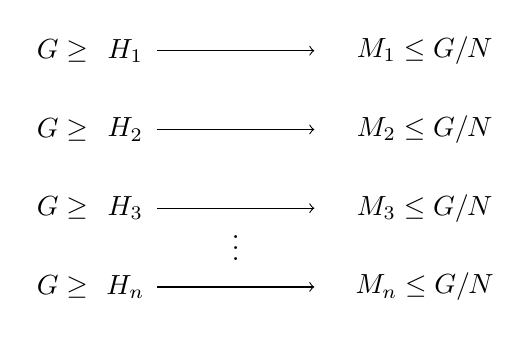
\begin{tikzpicture}
                \draw[->] (0,0) -- (2, 0);
                \draw[->] (0,-1) -- (2, -1);
                \draw[->] (0,-2) -- (2, -2);
                
                \node at (-0.4, 0) {$H_1$};
                \node at (-0.4, -1) {$H_2$};
                \node at (-0.4, -2) {$H_3$};
    
                \node at (3.4, 0) {$M_1 \le G/N$};
                \node at (3.4, -1) {$M_2 \le G/N$};
                \node at (3.4, -2) {$M_3 \le G/N$};

                \node at (-1.2, 0) {$G \ge $};
                \node at (-1.2, -1) {$G \ge $};
                \node at (-1.2, -2) {$G \ge $};
    
                \node at (1, -2.4) {$\vdots$};

                \node at (-0.4, -3) {$H_n$};
                \node at (3.4, -3) {$M_n \le G/N$};
                \node at (-1.2, -3) {$G \ge $};
                \draw[->] (0,-3) -- (2, -3);
                
            \end{tikzpicture}
        % \end{figure}
    \end{minipage}\hfill
    \begin{minipage}{0.55\textwidth}
        The Fourth Isomorphism Theorem is also commonly known as the
        correspondence theorem, since what it effectively states is that
        there is a one-to-one correspondence between subgroups $H$ of $G$
        which contain $N$ and the subgroups of $G/N$.

        Thus, if $G$ has $n$ subgroups $H_i$ which contain $N$, then $G/N$
        has $n$ subgroups.
    \end{minipage}


    \begin{prf}
        We first prove the first statement.

        \textcolor{NavyBlue}{Our goal here will be to show that $M \le
        G/N \implies M = H/N$ where $M$ is some subgroup of $G/N$ and
        $N \le H \le G$.} 
        \begin{description}
            \item[\phantom{1}]
            \hspace{0.5cm} Consider a subgroup $M$
            of $G/N$. Let $H$ be the set of all $h \in G$ such that
            $Nh \in M$. Then observe that $N \subset H$, since the smallest
            subgroup of $G/N$ is the trivial group, namely $\{N\}$.
            Therefore $N \subset H \subset G$.
            
            \textcolor{NavyBlue}{Now we
            show that $N \le H \le G$. To do this, we just need to
            show that $H \le G$, which we will do by the subgroup test.}

            Let $h, h' \in H$. Since $M \le G/N$, we know that for any
            $Nh, Nh' \in M$,  
            \[
                \underbrace{(Nh')(Nh)^{-1} \in M}_{\text{by the Subgroup Test}} \implies (Nh')(Nh^{-1}) \in M 
                \implies N(h'h^{-1}) \in M.
            \]
            However, in order for $N(h' h^{-1}) \in M$, we have that
            $h'h^{-1} \in H$. Since $h, h'$ were arbitrary elements of
           $H$, we have by the subgroup test we have that
            $H \le G$.  
            
            But since we have that $N \le G$, $H \le G$ and $N \subset
            H \subset G$, we all together have that $N \le H \le G$. 
        \end{description}
        Next, we prove the the statements $(1)-(4).$
        \textcolor{NavyBlue}{To prove (1), we'll show that $H/N \le K/N \implies H \le K$
        and $H \le K \implies H/N \le K/N$ for any subgroups $H, K$ of
        $G$ which contain $N$ where $N \normal G$.}

        \begin{description}
            \item[\phantom{1}]
            \hspace{0.5cm} Let $H, K$ be subgroups of $G$ such that $N
            \subset H$ and $N \subset K$. Furthermore, suppose that 
            $H/N \le K/N$.
            
        \end{description}
    \end{prf}

    
    The Isomophism Theorems are extremely powerful. The following
    an application to something which matches our intuiton, but
    extremely difficult to prove without the isomophism theorems.    
    \begin{thm}\label{product_theorem}
        Let $G$ be a group and $H$ and $K$ be normal subgroups of $G$.
        Then 
        \begin{itemize}
            \item[1.] $HK$ is a subgroup of $G$ 
            \item[2.] If $\gcd(|H|, |K|) = 1$ then $H \times K \cong
            HK$. 
        \end{itemize}
    \end{thm}

    \begin{prf}
        \begin{itemize}
            \item[1.] Observe that since $H \unlhd G$ and $K \unlhd G$, then obviously 
            $H \le G$ and hence we can apply the Second Isomorphism Theorem to conclude 
            that $HK \le G$. Thus we see that for this statement to be true in general 
            we really only need one of the subgroups, either $H$ or $K$, to be normal 
            to $G$.

            \textcolor{NavyBlue}{To prove this, we'll construct an
            isomorphism between the two groups. In constructing the
            homomorphism, we'll have to do a bit of work to show our
            proposed homorphism is in fact a homomorphism, the work
            which lies in showing elements of $H$ and $K$ commute.
            Thus we will show this first.}

            \item[2.]The fact that $\gcd(|H|,|K|)=1$ allows us to concldue that neither 
            $H \not \le K$ and $K \not \le H$, since otherwise by Lagrange's theorem 
            the order of one group would divide the other, and obviously we don't have 
            that case here. Thus we know that $H \cap K = \{e\}$, as by our previous 
            argument it would be impossible for them to share any other nontrivial element.
            \\
            \\
            Since $H, K$ are 
            normal to $G$ we'll have that 
            \begin{align*}
                hkh^{-1} \in K\\
                kh^{-1}k^{-1} \in H
            \end{align*}
            because $h$ and $k$ are both elements in $G$, and we know 
            for all $a \in G$ that $aha^{-1} \in H$ for $h \in H$ and 
            $aka^{-1} \in K$ for $k \in K$.
            We can then state that 
            \begin{align*}
                \overbrace{(hkh^{-1})}^{\text{A member of }K} \hspace{-0.3cm}k^{-1} = hkh^{-1}k^{-1} \in K\\
                h\underbrace{(kh^{-1}k^{-1})}_{\text{A member of } H} = hkh^{-1}k^{-1} \in H
            \end{align*}
            by using the fact that $H, K$ are subgroups and are therefore closed under products 
            of their elements. But we showed earlier that $H \cap K = \{e\}$; hence 
            $$
            hkh^{-1}k^{-1} \in H \cap K = \{e\} \implies hkh^{-1}k^{-1} = e \implies hk = kh.
            $$
            But $h, k$ were arbitrary elements of $H, K$, so this shows that products of 
            their elements commute.
            \\
            \\
            Next, consider the function $\phi: H \times K \rightarrow
            HK$ defined as
            $$
            \phi((h, k)) = hk.
            $$
            which we will 
            show to be a homomorphism.
            Observe that if $(h_1, k_1)$ and $(h_2, k_2)$ are in $H \times K$, then 
            $$
            \phi((h_1, k_1)\cdot(h_2, k_2)) = \phi((h_1h_2, k_1k_2)) = h_1h_2k_1k_2.
            $$
            However, we showed that products of elements between $H$ and $K$ can commute, so that 
            we can rewrite $h_2k_1$ as $k_1h_2$ to write 
            $$
            \phi((h_1, k_1)\cdot(h_2, k_2)) =  h_1h_2k_1k_2
            = h_1k_1h_2k_2 = \phi((h_1, k_2))\phi((h_2, k_2)).
            $$
            Thus $\phi$ is a homomorphism. \\
            \\
            Observe now that $\text{ker}(\phi) = \{(e, e)\}$. This is because we 
            know that $H \cap K = \{e\}$, so that if 
            $$
            \phi((h, k)) = hk = e
            $$
            we know it is impossible that this could be because $h = k^{-1}$; otherwise, 
            $H \cap K \ne \{e\}$, which we know is not the case. 
            Hence the only time when $hk = e$ is if both $h$ and $k$ 
            are $e$, so that $\text{ker}(\phi) = \{(e, e)\}$.
            \\
            \\
            Observe that $\text{im}(\phi) = HK$. This is because for any $hk \in 
            HK$, we can simply observe that $h \in H, k \in K$, and therefore there 
            exists a $(h, k) \in H \times K$ such that 
            $$
            \phi(h, k) = hk.
            $$
            Thus every element of $HK$ is covered by our mapping, so $\phi$ is injective 
            and hence $\text{im}(\phi) = HK$.
            \\
            \\
            Finally, what we have shown is that (1) $\phi$ is a homomorphism and 
            (2) it is a bijection from $H \times K$ to $HK$. We can now apply the 
            First Isomorphism Theorem to conclude that 
            $$ 
            H \times K/\text{ker}(\phi) \cong \text{im}(\phi) \implies H\times K \cong HK
            $$
            because $\text{ker}(\phi) = \{(e, e)\}, H \times K/\{(e, e)\} = H \times K$, 
            and $\text{im}(\phi) = HK$. This completes the proof.
        \end{itemize}
    \end{prf}

    The First Isomophism Theorem has a lot of fun applications, one of
    which we present here. 

    \begin{thm}
        Let $G$ and $H$ be groups such that $|G|$ and $|H|$ are
        coprime. If $\phi: G \to H$ is a homomorphism, then $\phi$ is
        zero homomorphism. 
    \end{thm}

    \begin{prf}
        By the First Isomorphism Theorem, we see that 
        \[
            G/\ker(\phi) \cong \im(\phi).   
        \]
        Therefore $|G/\ker(\phi)| = |\im(\phi)|$. However, 
        \begin{align*}
            |G/\ker(\phi)| = |G|/|\ker(\phi)| &= |\im(\phi)|\\ 
            \implies |G| &= |\ker(\phi)| \cdot  |\im(\phi)|.
        \end{align*}
        Note that $|\ker(\phi)| \mid |G|$ and $|\im(\phi)| \mid |H|$ by
        Lagrange's Theorem. However, we said that $|G|$ and $|H|$ are
        corpime
        which means that $|\im(\phi)| = 1$. Hence we
        must have that $|\ker(\phi)| = G$, and since $\ker(\phi) \le G$ we
        have that $\ker(\phi) = G$. Therefore $\phi$ sends every element
        of $G$ to the identity of $H$, which is what we set out to show.
    \end{prf}


    \newpage
    \section{Group Actions.}
    As we shall see, a group action is a special type of mapping one can
    formulate involving a group $G$ and an arbitrary set of objects $X$.
    Specifically, it is a mapping from $G \times X \to X$.
    Thus, a group action is said to make a group $G$ "act" on a set
    $X$. It is through this perspective that one can then view group
    actions as permutations of a set $X$. This becomes more clear with
    the formal definition. 

    \begin{definition}
        Let $G$ be a group and $X$ an arbitrary set. A \textbf{group
        action} of $G$ on $X$ is a mapping $* : G \times X \to X$
        that 
        \begin{itemize}
            \item[1.] $g_1 * (g_2 * x) = (g_1 \cdot g_2) * x$ for
            all $g_1, g_2 \in G, x \in X$.

            \item[2.] $e * x = x$ where $e \in G$ is the identity.
        \end{itemize}
    \end{definition}
    Note that $\cdot$ is the \textit{group multiplication in $G$.} For
    notational convenience, we will surpress $\cdot$ in the cases for
    where it's obvious or implied, as usual.
    \\
    We also note that we could have defined $*:X \times G \to X$. For
    simplicity, we let $G$ act on the left.
    \\  

    Let's breakdown what this is really saying.
    \textcolor{red}{For a group
    action $*$ of $G$ acting on $X$, we have for all $g \in G$, $x \in
    X$, the product $g * x$ is mapped to some element $x' \in X$.}

    Now observe that if
    we replaced $X$ with $G$, then we get $* : G \times G \to G$.
    Thus $*$ would just permutate the elements of $G$.
    Furthermore, if we let $*$ be the group multiplication $\cdot$ which
    is already defined in $G$, then we just get back the definition of
    a group! 
    
    \textcolor{NavyBlue}{This fits with the intuition that,
    group multiplication of elements (e.g., $g \cdot g'$ where $g, g'
    \in G$) simply permutates the elements of a group. That is, if 
    you placed the elements of $G$ in a tuple such as 
    \[
        (g_1, g_2, \dots, g_n)
    \] 
    and multiplied this by some $g' \in G$, you would get a tuple 
    \[
        (g_1, g_2, \dots, g_n) \cdot g' 
        = (g_1\cdot g', g_2 \cdot g' , \dots, g_n\cdot g')
        =
        (g_i, g_j, \dots, g_k)
    \]
    containing all the elements of $G$, but just in a different order.
    (In this case we supposed $g_1 \cdot g' = g_i, g_2, \cdot g' =
    g_j$, and so on.)
    } 

    \begin{minipage}{0.7\textwidth}
        \vspace{.3cm}
        This permutation phenonmenon can be found in more general
        group actions.  For a fixed $g \in G$, define $\sigma_g:
        X \to X$ as 
        \[
            \sigma_g(x) = g * x.
        \] 
        So $\sigma_g$ maps each $x$ to some other element $x' \in X$.
        Therefore, a group action can be thought of as a set of maps
        $\sigma_g$, one for every element $g \in G$, each of which can
        appropriately be composed with one another. 
        
        That's why
        it can be thought of as a permutation. The diagram on the right
        gives an illustration how this plays out for one particular
        $g \in G$ acting on a set $X$ with five elements.
    \end{minipage}\hfill
   \begin{minipage}{0.2\textwidth}
        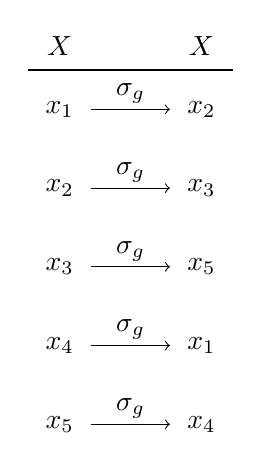
\begin{tikzpicture}
            \draw (-0.8,0.5)--(1.8,0.5);
            \draw[->] (0,0) -- (1,0);
            \draw[->] (0,-1) -- (1,-1);
            \draw[->] (0,-2) -- (1,-2);
            \draw[->] (0,-3) -- (1,-3);
            \draw[->] (0,-4) -- (1,-4);

            \node at (-0.4, .8) {$X$};
            \node at (-0.4, 0) {$x_1$};
            \node at (-0.4, -1) {$x_2$};
            \node at (-0.4, -2) {$x_3$};
            \node at (-0.4, -3) {$x_4$};
            \node at (-0.4, -4) {$x_5$};

            \node at (0.5, 0.2) {$\sigma_g$};
            \node at (0.5, -0.8) {$\sigma_g$};
            \node at (0.5, -1.8) {$\sigma_g$};
            \node at (0.5, -2.8) {$\sigma_g$};
            \node at (0.5, -3.8) {$\sigma_g$};
            
            \node at (1.4, 0.8){$X$};
            \node at (1.4, 0) {$x_2$};
            \node at (1.4, -1) {$x_3$};
            \node at (1.4, -2) {$x_5$};
            \node at (1.4, -3) {$x_1$};
            \node at (1.4, -4) {$x_4$};
            
        \end{tikzpicture}
        
    \end{minipage} 
    \vspace{.5cm}

    \textcolor{NavyBlue}{Here's another way to think about a group
    action. If $G$ acts on $X$, then the group action $*$ turns each 
    and every element of $g \in G$ into a \textit{function}, which
    maps $X$ to $X$. This agrees with our intuition, since a
    permutation is exactly a function of $X$ to itself. }
    \begin{thm}
        A finite group of order $n$ is isomorphic to a subgroup of $S_n$.
    \end{thm}
    
    This theorem is a powerful theorem that gives us a new way to
    think about finite groups. It states that every finite group is
    basically the same as a subgroup of a symmetric group up to an
    isomorphism. 

    \begin{prf}
        \textcolor{NavyBlue}{To prove this, we'll first construct a
        group action of $G$ on itself. Then we'll }

        Consider the group action of $G$ acting on itself, whereby we
        define $g_1 \cdot g_2 = g_1g_2$ for $g_1, g_2 \in G$. That is,
        the group action 
        mapping is simply the multiplication used between the elements
        of $G$. 
        \begin{description}
            \item[This is a Group Action.] 
            (Note: we already pointed out that if we replace $X$ with
            $G$ in the definition of a group action, and let $\cdot$
            be the group multiplication in $G$, then we just get the
            definition of a group. Thus a group is a special, but
            boring, type group action.)

            To show this is a group action, let $x \in G$. Then 
            \[
                g_1 \cdot (g_2 \cdot x) = g_1 \cdot (g_2x) = g_1g_2x = (g_1g_2)x = (g_1g_2) \cdot x.
            \]
            for $g_1, g_2 \in G$.
            Therefore, $g_1 \cdot (g_2 \cdot x) = (g_1g_2) \cdot x.$
            The second axiom is satisfied, since if $e$ is the
            identity of $G$, then clearly $e \cdot x = ex = x$. We
            have both axioms satisfied. So this is a group action. 
        \end{description}
    \end{prf}

    Before we lead up to a powerful theorem involving group actions,
    we must define a few definitions. 
    
    \begin{definition}
        Suppoe $G$ acts on a set $X$, and let $x \in X$. Then we
        define the set 
        \[
            Gx = \{g * x \mid g \in G \}
        \]
        as the \textbf{orbirt} of $x$. 
    \end{definition}

    The orbit basically considers the set of all images one obtains
    when one grabs a single element of $x \in X$, and multiplies it by
    every element $g \in G$. {\color{purple}{Note that since $g
    \cdot x \in X$ for every $g \in G, x \in X$, we have that $Gx \subset X$.}}
    
    \textcolor{NavyBlue}{Orbits are rather interesting since \textbf{they partition their acting
    set $X$}. That is, if $X = \{x_1, x_2, \dots, x_n\}$, then 
    $Gx_1 \cup Gx_2 \cup \cdots \cup Gx_n = X$. Note that $x_i \in
    Gx_i$ for $i = 1, 2, \dots, n$, so this definitely makes sense.
    \\
    \\
    However, it is possible that $Gx_i = Gx_j$ for some $i, j.$ In
    such a case we note that for each $g \in G$ there exists a $g' \in
    G$ such that $gx_i = g'x_j \implies g^{-1}g'x_j = x_i$. Since
    $g^{-1}g' \in G$, 
    our condition boils down to the following: 
    $Gx_i = Gx_j$ for some $i, j$ if there exists a $g \in G$
    such that 
    $gx_j = x_i$. So $Gx_i = Gx_j$ if $x_j \in Gx_i$.}
    \\
    \\
    Thus, these things are behaving like cosets (recall that $Gh =
    Gh'$ if and only if $h' \in Gh$.) and they partition the acting
    set $X$! This understanding will become helpful in the future. 
    \\
    \\
    Since orbits form partitions, and it is possible that the set of
    all orbits will be redundant (i.e., it's possible that $Gx_i =
    Gx_j$ for some $i, j$), we offer the following definition.

    \begin{definition}
        Let $G$ be a group, and suppose it acts on a set $X$. 
        Let $Gx_1, Gx_2, \cdots, Gx_n$ be a distinct set of
        orbits  such that 
        \[
            Gx_1 \cup Gx_2 \cup \cdots G_n = X.
        \]
        Then each $x_1, x_2, \dots, x_n$ are called
        \textbf{representatives of an orbit} of $G$. We generally
        denote $R = \{x_1, x_2, \dots x_n\}$ to be the set of
        representatives of the orbits. 
    \end{definition}

    Thus for some orbit $Gx_i$, we say that $x_i$ "represents" this
    orbit. We make this definition since we just showed that 
    it doesn't really matter what representative we pick, since if 
    $x_j \in Gx_j$, $Gx_j = Gx_i$, so $x_j$ could have equally
    represented this orbit. Thus given this arbitrary-ness, the
    definition allows us to talk about orbits more easily.
    
    We now offer another definition regarding group actions.

    \begin{definition}
        Suppose $G$ acts on $X$, and $x \in X$. Then the set 
        \[
            G_x = \{g \in G \mid g * x = x\}.
        \]
        is defined to be the \textbf{stabilizer} of $x$.
    \end{definition}
    
    The stabilizer considers the elements of $g \in G$ which act as an
    identity to $x$. \textcolor{purple}{Since $G_x$ considers elements
    of $G$, we see that $G_x \subset G$. Furthermore, we have the
    following proposition.}

    \begin{proposition}
        Suppose $G$ acts on $X$, and let $x \in X$. Then $G_x \le G$.
    \end{proposition}

    \begin{prf}
        Observe first that this is nonempty, since $e * x = x$ for
        all $x \in X$, where $e \in G$ is the identity. Therefore $e
        \in G_x$. Next, observe that associativity is inherited from
        the set $G$ itself. To check for inverses, we note that for any $g \in G$, $g \cdot x = x$, 
        so we can multiply both sides by $g^{-1}$ to get
        \[  
            g^{-1} * g * x = g^{-1} * x \implies (g^{-1}g) * x = g^{-1} * x 
            \implies x = g^{-1} * x.
        \]
        Thus $g^{-1} * x = x$ so $g^{-1} \in G$. Finally, observe
        that the set is closed. Given $g, g' \in G_x$, we see that 
        \[
            (gg') * x = g * (g' * x) = g *`' (x) = x.
        \]
        Therefore $G_x$ is (1) a subset of $G$ and (2) a group so it
        is a subgroup of $G$.

    \end{prf}
    We now move onto one of the useful theorems that arises once one
    realizes the definitions of the orbit and stabilizers.

    \begin{thm}
        Let $G$ be a finite group, and suppose $G$ acts on a set $X$.
        Then for any $x \in X$ we have that 
        \[
            |G| = |Gx| \cdot |G_x|.
        \]
    \end{thm}

    \begin{prf}
        To show this, we'll construct a bijection between $Gx$ and
        $G/G_x$. 

        Let $g \in G$ so that $gG_x \in G/G_x$. Then construct the map
        $\psi: G/G_x \to Gx$ by
        \[
            \psi(gG_x) = g * x.
        \]
        Note that there is only one element in $G/G_x$ which gets
       to $x$; namely, $G_x$. The calculation is as follows:
       \[
            \psi(G_x) = e * x = x.
       \]
       This map is obviously surjective, since for any $x' \in Gx$, we
        we know that there exists a $g \in G$ such that $g * x = x'$.
        Thus $g \not\in G_x$, so that $gG_x$ is nontrivial and
        $\psi(gG_x) = g * x = x'$.

        Now to show that this is injective, suppose that $g*x = h*x$.
     we have that $g^{-1}h * x = x$. Therefore, $gh^{-1} \in G_x$.
     Furthermoresee that 
     \[
         g^{-1}hG_x = G_x \implies hG_x = gG_x.
     \]
     Thus this can only happen if the input is the same. Therefore
     this is a one-to-one and onto mapping. 

     Since this is a bijection, we can conclude that 
     \[
        |Gx| = |G/G_x| = |G|/|G_x| \implies |G| = |Gx||G_x|    
     \]
     as desired.
    \end{prf}
    

    \newpage
    \section{Conjugation, The Class Equation, and Cauchy's Theorem.}
    \textcolor{blue}{We now touch on a very deep example of a group action, known as
    conjugation.} Let $G$ act on itself "by conjugation", which we define
    as follows. Let $g, h \in G$. Then 
    \[
        g * h = ghg^{-1}
    \]
    is the group action of conjugation.
    Let's show that this is a group action. 
    \begin{description}
        \item[Composition.] Let $g_1, g_2, h \in G$. Then observe that
        \begin{align*}
            g_1 * (g_2 * h) = g_1 * (g_2hg_2^{-1}) &= g_1g_2 h g_2^{-1}g_1^{-1} \\
            & = (g_1g_2) h (g_1g_2)^{-1} \\
            & = (g_1g_2) * h
        \end{align*}
        so that the first axiom of a group action is satisfied.
        \item[Identity.]
        Observe also that for $e \in G$, the identity of $G$, 
        \[
            e * h = ehe^{-1} = h.
        \]
        Therefore this is a group action.
    \end{description}

    We'll now show that this group action is very special and
    important. Conjugation itself is important in math. In Linear
    Algebra, two matrices which are similar (i.e., $A$ is similar to
    $B$ if there exists $P$ such that $A = P^{-1}BP$) have \textbf{the same 
    rank, determinants, trace, eigenvalues, and much more}. Basically,
    they represent the same linear transformation, just in different
    bases. To learn more about conjugation, we make a few definitions
    with this group action.

    \begin{definition}
        Let $G$ be a group, and let $G$ act on itself by conjugation.
        For any $h \in G$, \textbf{the orbit} of this group action
        \begin{align*}
            Gh & = \{g * h \mid g \in G\} \\
            & = \{ghg^{-1} \mid g \in G\}
        \end{align*}
        is known as a \textbf{conjugacy class} of $G$.
    \end{definition}

    \textcolor{purple}{Previously we discussed how orbits of a group action partition the
    set $X$ which is being acted on. Since $G$ acts on itself in this
    example, we see that \textbf{the conjugacy classes form a
    partition of $G$!}}
    \\
    \\
    \textbf{Remark.}
    Recall the definition of a centralizer $G$ for a set $A \subset
    G$: 
    \begin{align*}
        C_G(A) & = \{g \in G \mid gs = sg \text{ for all } s \in S\}\\
        & = \{g \in G \mid gsg^{-1} = s  \text{ for all } s \in S\}.
    \end{align*}
    Therefore for a single point $x \in G$, $C_G(x) = \{g \in G \mid
    gxg^{-1} = x \} = \{g \in G \mid g * x = x\}$, where in the last
    equation we are speaking in terms of group actions. But note that
    this last set is exactly the \textbf{stabilizer} of $G$ under this
    group action. \textbf{\textcolor{NavyBlue}{Therefore, $C_G(x) = G_x$ for any $x \in G$ under
    this group action.}}

    Furthermore, let $x \in Z(G) = \{z \in G \mid z = gzg^{-1} \text{
    for all } g \in G\},$ the center of $G$. Then we see that $Gx =
    \{gxg^{-1} \mid g \in G\} = \{x\}$. \textbf{\textcolor{NavyBlue}{So for any $x \in Z(G)$, the
    orbit is of size one. The sole element it contains is just $x$.}} (We can go even further: the conjugacy
    classes of an abelian group are all of size one.)
    \\
    \\
    Let's put all of these results together. In general, if $G$
    acts on itself via conjugation, then we know its orbits, or
    conjugacy classes, partition $G$. Moreover, let $R \subset X$ be a set of
    orbit representatives (or conjugacy class representatives, if you
    like). Then 
    \[
        |G| = \sum_{x \in R}|Gx|
    \]
    Recall that $|Gx| = 1$ if $x \in Z(G)$. Thus we can write this
    further as 
    \begin{align*}
        |G| = 
        \sum_{x \in Z(G)}|Gx| + \sum_{x \in R\setminus Z(G)} |Gx|
        & = \sum_{x \in Z(G)}1 + \sum_{x \in R\setminus Z(G)} |Gx|\\
        & = |Z(G)| + \sum_{x \in R\setminus Z(G)} |Gx|
    \end{align*}
    By the Orbit-Stabilizer theorem, we can write $|Gx| = |G|/|G_x|$.
    Substituting this in, we get 
    \begin{align*}
        |G| &= |Z(G)| + \sum_{x \in R\setminus Z(G)} |G|/|G_x|
    \end{align*}
    and since $C_G(x) = G_x$,
    \begin{align*}
        |G| = |Z(G)| + \sum_{x \in R\setminus Z(G)} |G|/|C_G(x)|
    \end{align*}
    which is known as the \textbf{class equation.} This equation is
    pretty badass, as it gives us a way to understand the cardinality
    of a group. This equation is also useful in proofs, as we shall
    see in the following examples. First, we begin with a lemma. 

    \begin{lemma}
        Let $G$ be a group. Then $C_G(x) = G$ if and only if $x \in Z(G)$.
    \end{lemma}

    \begin{prf}
        Suppose $C_G(x) = G$. Then for all $g \in G$, $gx = xg$.
        However, $Z(G)$ is the set of all $G$ which commutes with
        every member of $G$, so $x \in Z(G)$. 
        Now suppose $x \in Z(G)$. Then $gx = xg$ for all $g \in G$.
        Therefore, $C_G(x) = \{g \in G \mid gx = xg\} = G$.
    \end{prf}

    \begin{thm} \label{center_lemma}
        Let $G$ be a group such that $|G| = p^n$ for some prime $p$
        and $n \in \mathbb{N}$. Then $|Z(G)| > 1$. That is, $|Z(G)|
        \in \{p, p^2, \dots, p^{n}\}$.
    \end{thm}
    \textcolor{Purple}{Equivalently, this theorem says that $Z(G)$ is nontrivial.
    Moreover, this implies that \textbf{there exists
    non identity elements of $\mathbf{G}$ which commute with every
    element of $\mathbf{G}$.}}

    \begin{prf}
        First observe that $Z(G)$ is a subgroup of $G$. Therefore, by
        Lagrange's Theorem, we know that $|Z(G)|$ divides $G$. Thus
        $|Z(G)| \in \{1, p, p^2, \dots, p^{n}\}$. Our goal is to show
        that $|Z(G)|$ cannot equal 1.

        \textcolor{NavyBlue}{For the sake of contradicton, suppose $|Z(G)| = 1$}. Then by
        the previous lemma, we see that 
        there is no nontrivial element $g$ of $G$ such $C_G(g) = G$.

        Let $R$ be the set of conjugacy class representatives. 
        Then $|G|/|C_G(r)| \in \{p, p^2, \cdots, p^n\}$ for $r \in
        R\setminus Z(G)$ (since $|Z(G)| = 1$, $R\setminus Z(G)$ simply
        removes $e$, the identtiy, from $R$).

        \textcolor{red!40!purple!100}{Why can't $|G|/|C_G(r)| = 1$ for any $r \in
        R\setminus Z(G)$? Well, because for such an $r$, $r \not\in
        Z(G)$. Therefore $C_G(r) \ne G$, so $|G|/|C_G(r)| \ne 1$.}

        Now by the class equation, we see that 
        \[
            \underbrace{ \hspace{.2cm}|G|\hspace{.2cm}   }_{\text{divisible by } p} \hspace{-.5cm} = |Z(G)| + \overbrace{\sum_{r \in R\setminus Z(G)} |G|/|C_G(r)|}^{\text{divisible by } p}
        \]
        since $|G|/|C_G(r)| \in \{p, p^2, \dots, p^n\}$ for all $r \in
        R\setminus Z(G)$. \textcolor{NavyBlue}{Therefore we see that $|Z(G)|$ must be
        divisible by $p$. But this is a contradiction since we said
        $|Z(G)| = 1$}. Therefore, we see that $|Z(G)| \in \{p, p^2,
        \dots, p^n\}$.
        
    \end{prf}

    The above theorem can be used to prove the next theorem, whose
    signifiance demonstrates the power of the class equation.
    The theorem below is generally
        proved by proving the above theorem first in the special case
        for when $|G| = p^2$. But it will be helpful to other proofs
        later on to consider the more general case as we presented it above.

    \begin{thm}
        Let $G$ be a group, and suppose $|G| = p^2$ where $p \ge 2$ is
        prime. Then $G$ is abelian. 
    \end{thm}

    \begin{prf}
        \textcolor{green!50!black}{By the previous theorem, we see
        that $|Z(G)| \in \{p, p^2\}$.)} We'll proceed by considering two cases.

        \begin{description}
            \item[$\mathbf{|Z(G)| = p^2}$.] 
            In this case $|G| = |Z(G)|$. Since we also have that
            $Z(G)$ is a subgroup of $G$, we can conclude that $G =
            Z(G)$. 
            Therefore, $G$ is abelian. 
             
            \item[$\mathbf{|Z(G)| = p}$.] 
            Recall that $Z(G) \normal
            G$ from Proposition \ref{normal_center}. Therefore, we can
            speak of the quotient group $G/Z(G)$, which has size
            $|G|/|Z(G)| = p^2/p = p$. By the corollary to Lagrange's
            Theorem, this implies that $G/Z(G)$ is cyclic, since it
            has prime order. Thus there
            exists a $g \in G$ such that we can represent $G/Z(G)$ as 
            \[
                G/Z(G) = \{Z(G), Z(G)g, Z(G)g^2, \dots, Z(G)g^{p-1}\}.
            \]
            As we already know, cosets partition $G$. Therefore, let
            $a, b \in G$, and suppose $a \in Z(G)g^i$ and $b \in
            Z(G)g^j$. Then there exist $x, y \in Z(G)$ such that 
            $a = xg^i$ and $b = yg^j$. Thus observe that 
            \begin{align*}
                ab = xg^i yg^j = xyg^ig^j = xyg^{i+j} = xyg^jg^i
                = yg^jxg^i = ba
            \end{align*}
            where we used the commutavity of $x,y$ since $x, y \in
            Z(G)$. Since $a, b$ were arbitrary members of $G$, this
            proves that $G$ is abelian.
        \end{description}
    \end{prf}

    Thus we see that the class equation is useful in proving more
    general facts about group theory. The class equation can also be
    used to prove the following important theorem in group theory,
    known as Cauchy's Theorem. 

    \begin{thm}[ (Cauchy's Theorem)]
        Let $G$ be a finite group and $p \ge 2$ be a prime. If $p$ divides
        the order of $G$, then $G$ has an element of order $p$. 
    \end{thm}

    \noindent\textcolor{NavyBlue}{So consider a group $G$ with order $n$,
    and suppose 
    \[ n = p_1^{i_1}\cdot p_2^{i_2} \cdots
    p_n^{i_n}
    \]
    is its prime factorization. Then there exist elements
    $g_1, g_2, \dots, g_n$ such that $|g_i| = p_i$ for $i = 1, 2,
    \dots, n$.}

    Another way to visualize this as follows. Consider a group $G$
    consisting of 10 elements. 
    \[
        \{e, \hspace{.1cm}g_1,\hspace{.1cm} g_2,\hspace{.1cm} g_3,\hspace{.1cm} g_4,\hspace{.1cm} g_5,\hspace{.1cm} g_6,\hspace{.1cm} g_7,\hspace{.1cm} g_8,\hspace{.1cm} g_{9}\}
    \]
    By Cauchy's theorem, there exists elements of order $2$ and $5$.
    So suppose $g_1$ and $g_2$ are such elements, i.e., $g_1^2 = 3$
    and $g_2^5 = e$. Then we can really rewrite this as 
    \[
        \{e,\hspace{.1cm} \textcolor{red}{g_1},\hspace{.1cm} \textcolor{blue}{g_2},\hspace{.1cm} \textcolor{blue}{g_2^2},\hspace{.1cm} \textcolor{blue}{g_2^3},\hspace{.1cm} \textcolor{blue}{g_2^4},\hspace{.1cm} g_6,\hspace{.1cm} g_7,\hspace{.1cm} g_8,\hspace{.1cm} g_9\}.   
    \] 
    However, we know $\textcolor{red}{g_1}\textcolor{blue}{g_2}, \textcolor{red}{g_1}\textcolor{blue}{g_2^2}, \textcolor{red}{g_1}\textcolor{blue}{g_2^3}$ and $\textcolor{red}{g_1}\textcolor{blue}{g_2^4}$ are all in $G$. Thus
    we can really write this as 
    \[
        \{e, \hspace{.1cm} \textcolor{red}{g_1},\hspace{.1cm} \textcolor{blue}{g_2},\hspace{.1cm} \textcolor{blue}{g_2^2},\hspace{.1cm} \textcolor{blue}{g_2^3},\hspace{.1cm} \textcolor{blue}{g_2^4}, \hspace{.1cm}\textcolor{red}{g_1}\textcolor{blue}{g_2},\hspace{.1cm} \textcolor{red}{g_1}\textcolor{blue}{g_2^2},\hspace{.1cm} \textcolor{red}{g_1}\textcolor{blue}{g_2^3},\hspace{.1cm} \textcolor{red}{g_1}\textcolor{blue}{g_2^4}\}.
    \] 
    Thus we can understand the structure of every single group of
    order 10. But this can be done for all finite groups!
    
    \begin{prf}
        \textcolor{Plum}{In this proof, we'll prove this in a very
        clevery way by letting a subgroup of a permutation group act
        on a special set $X$ (both of which we will define). This will then prove the existence of
        elements of order $p$.}

        Let $p$ be a prime which divides $|G|$. 
        Define $H$ to be the cyclic subgroup of $S_p$ generated by
        $(1\hspace{.1cm}2\hspace{.1cm}\cdots\hspace{.1cm}p)$. 

        We can picture $H$ as the group 
        \[
            \{(1\hspace{.1cm}2\hspace{.1cm}\cdots\hspace{.1cm}p), (2\hspace{.1cm}3\hspace{.1cm}\cdots\hspace{.1cm}p, \hspace{.1cm}1), \cdots, (p\hspace{.1cm}1\hspace{.1cm}\cdots\hspace{.1cm}p-1)\}.
        \]

        Now let $H$ act on the set $X$ defined as 
        \[
            X = \{ (g_1, g_2, \dots, g_p) \mid g_1, g_2, \dots, g_p \in G \text{ and } g_1g_2\cdots g_p = e \}
        \]
        where the $\sigma \in H$ acts on $g \in X$ as 
        \[
            \sigma \cdot (g_1, g_2, \dots, g_p) = (g_{\sigma(1)}, g_{\sigma(2)}, \dots, g_{\sigma(p)}).
        \]
        This $H$ takes a $p$-tuple in $X$ and permutates the elements.
        Since $H$ is generated by
        $(1\hspace{.1cm}2\hspace{.1cm}\cdots\hspace{.1cm}p)$, it
        "pushes" the elements $g_i$ in the tuple over to the right, and the elements
        that are pushed out of the right end of the tuple are pushed back in on
        the left side.

        \textcolor{NavyBlue}{First we'll show that this is a group action.}
        \begin{description}
            \item[This is a Group Action.] 
                Let $x \in X$ and $\sigma \in H$. If $x = (g_1, g_2,
                \dots , g_p)$, observe that 
                \[
                    \sigma * x = (g_{\sigma(1)}, g_{\sigma(2)}, \dots, g_{\sigma(p)}).
                \]
                Suppose $h(1) = n$. Then in general $h(i) = (i + n)
                \mbox{ mod }p.$ Therefore, we see that 
                \[
                    (g_{\sigma(1)}, g_{\sigma(2)}, \dots, g_{\sigma(p)}) 
                    = 
                    (g_{n}, g_{n+1}, \dots, g_p, g_1, \dots, g_{n-1}).
                \]
                However, observe that 
                \[
                    g_1g_2\cdots g_p = g_1g_2 \cdots g_{n-1}g_n g_{n+1} \cdots g_p = e
                    \implies (g_1g_2 \cdots g_{n-1})(g_n g_{n+1} \cdots g_p) = e.
                \]
                Thus the elements $g_1g_2 \cdots g_{n-1}$ and $g_n
                g_{n+1} \cdots g_p$ in $G$ are inverses of each other. But
                know that if two group elements are inverses, either order
                of their product returns $e$. Therefore 
                \[
                    (g_ng_{n+1} \cdots g_{p})(g_1g_2 \cdots g_{n-1}) 
                    = g_ng_{n+1} \cdots g_{p}g_1g_2 \cdots g_{n-1} = e.
                \]
                                
                We therefore see that
                $(g_{n}, g_{n+1}, \dots, g_p,
                g_1, \dots, g_{n-1}) = \sigma *x \in X$. 

                Now we verify associativity. For any $\sigma_1,
                \sigma_2 \in H$, we see that 
                \begin{align*}
                    \sigma_1 * \sigma_2*x &= \sigma_1 * (g_{\sigma_2(1)}, g_{\sigma_2(2)}, \dots, g_{\sigma_2(p)})\\
                    &= (g_{\sigma_1(\sigma_2(1))}, g_{\sigma_1(\sigma_2(2))}, \dots, g_{\sigma_1(\sigma_2(p))})\\
                    &= (\sigma_1 \sigma_2) * (g_1, g_2, \dots, g_p).
                \end{align*}
                Thus $*$ is associative. Finally, if $\sigma$ is the
                trivial element, 
                \[
                    \sigma * x = (g_{\sigma(1)}, g_{\sigma(2)}, \cdots g_{\sigma(p)}) = (g_1, g_2, \dots, g_p) = x.
                \]
                Therefore this is a group action.
        \end{description}
        \textcolor{NavyBlue}{Now that we've shown that this is a group
        action, we'll argue that the orbits are either of size 1 or
        $p$.}
        
        \begin{description}
            \item[The Orbits.] 
            For any $x \in X$ such that $x = (g_1, g_2, \dots, g_p)$,
            we see that the orbit $Hx$ will simply be all of
            the permutations of the $p$-tuple $(g_1, g_2, \dots,
            g_p)$. Note however that there are only $p$ many ways to
            rearrange this tuple, so that any orbit $Hx$ will be of
            size $p$.

            Of course, the exception to this is if $g_1 = g_2 = \dots = g_p$. In
            this case, there are no other ways to reorganize the
            tuple. Hence the orbit will have size 1.
        \end{description}

        \textcolor{NavyBlue}{Finally, we will show that there exists a
        nontrivial orbit of size 1. This is equivalent to show that
        there exists a nontrivial element of $G$ of order $p$, which
        we'll eloaborate later.}

        \begin{description}
            \item[Orbit of Size 1.]
            First let's count the elements of $X$. Observe that for
            any $(g_1, g_2, \dots, g_p) \in
            X$, the last element $g_p$ is always determined by the
            first $p-1$ elements. This is because if we know the first
            $p-1$ elements, then 
            \[
                g_p = (g_1g_2 \cdots g_{p-1})^{-1}
            \]
            in order for $g_1g_2\cdots g_p = e$. Since there are
            $|G|^{p-1}$ many ways to pick the first $p-1$ elements in
            any $p$-tuple of $X$, we see that $X = |G|^{p-1}$. 

            Now by hypothesis, $p$ divides $|G|$. Therefore $p$
            divides $|X|$ so we may write $|X| = np$ for some integer $n$.

            Since the orbits of $X$ form a partition, the orbits
            partition a set $np$ elements into orbits of size $1$ or
            size $p$. We know one orbit of size 1 exists (namely, the
            trivial orbit $He = \{(e, e, \dots, e)\}$), so there must
            exist at least $p-1$ nontrivial other orbits of size 1. 

            Let $Hx'$ be one of those orbits. Then for some $g \in G$
            we have that $Hx = \{(g, g, \dots, g)\}$. However since
            $Hx \subset G$, what we have prove is the existence of a
            nontrivial
            element $g \in G$ such that $gg\cdots g = g^p = e$, which
           set out to show.
        \end{description}
        This completes the proof.
    \end{prf}
    Cacuhy's Theorem is an incredibly useful tool one can use in
    finite group theory. Here's an amazing and useful theorem who's
    proof is eased via Cauchy's Theorem.

    \begin{thm}
        Let $G$ be a group $p \ge 2$ a prime. If $|G| = p^n$ for some
        $n \in \mathbb{N}$, then $G$ has a subgroup of order $p^k$ for
        all $0 < k < n$.
    \end{thm}
    Note we didn't write $ 0 \le k \le n$. We could have, but we already
        know that there exists a subgroup of order $p^n$ (namely, $G$
        itself) and that there exists a subgrou of order $p^0 = 1$
        (namely, the trivial group).
    \begin{prf}
        \textcolor{NavyBlue}{To prove this, we'll use strong induction
        on the statement. Specifically, we'll induct on the powers of
        $n$.}

        Let us induct on $n$ in the statement above. Then for $n = 1$,
        there is no such $k < n$. Hence the statement is vacuously
        true. 

        Next suppose that the statement is true up to order $p^n$, 
        and let $G$ be a group of order $p^{n+1}$. 

        By Theorem 1.\ref{center_lemma}, we already note that $|Z(G)| >
        1$ and hence is a multiple of $p$. By Cauchy's Theorem, we
        then know that $Z(G)$ contains an element $g$ of order $p$.
        Note that (1) $\left< g\right>$ is a subgroup of $Z(G)$ and
        (2) $h\left< g \right> = \left< g \right>h$ for all $h \in G$
        (since, by definition of the center, every element of $Z(G)$
        commutes with elements of $G$). Therefore $\left< g \right>
        \normal G$. 

        Let $H = \left< g \right>$. Since we just showed $H \normal G$
        we can appropriately discuss the quotient group $G/H$.

        Observe that $|G/H| = |G|/|H| = p^{n+1}/p = p^n$. \textcolor{purple}{Thus by hypothesis, $G/H$ has a
        subgroup of order $p^k$ for all $0 < k < n$. Denote these such
        subgroups of $G/H$ as}
        \[
            \{N_1/H, N_2/H, \cdots N_{n-1}/H\}
        \]
        \textcolor{purple}{where $|N_k/H| = p^k$.}
        Since $H \normal G$, we
        know by the Fourth Isomorphism Theorem that every subgroup of
        $G/H$ is of the form $N/H$ where $H \le N \le G$. Thus we see
        that 
        \[
            H \le N_k \le G
        \]
        for all $0 < k < n$. But since $|N_k/H| = p^k$, and $|H| = p$,
        we see that each such $N_k$ will now have order $p^{k+1}$.
        Thus what we have shown is that $G$ itself contains subgroups
        of order $k$ for all $1 < k < n+1$. The subgroup $H$ of order
        $p$ is the final piece to this puzzle, and allows us to
        confirm that $G$ has a subgroup of order $p^k$ for all $0 < k < n$.
        By strong induction this holds for all $\mathbb{N}$,
        which completes the proof.
    \end{prf}



    \newpage
    \section{Sylow Theorems.}
    Lagrange's Theorem states that $H \le G$, then $|H|$ divides
    $|G|$. However, you may wonder if there is some kind of converse.
    If $k$ divides $|G|$, is there a subgroup of order $k$? 

    By Cauchy's Theorem, we know that if $p$ is a prime which divides
    then there exists an element of order $p$. Can we generalize this
    result further (for example, state \textit{how} many such elements
    satisfy this)? 

    The answer to both questions is yes and is achieved through
    Sylow's Theorem. It's a foundational theorem in finite group
    theory, as it
    strengthens our two most power theorems for finite groups:
    Lagrange's Theorem and Cauchy's Theorem.

    \begin{definition}
        $H$ is a \textbf{$p$-subgroup} of a group $G$ if $H$ is a
        subgroup of $G$ and $|H| = p^n$ for some $n \ge 1$.
    \end{definition}

    \begin{definition}
        Let $G$ be a group and let $p$ be a prime such that $p\mid
        |G|$. Suppose $p^k$ is the largest power such that $p^k \mid
        |G|$. That is, $|G| = p^km$ for some integer $m \in G$,
        $\mbox{gcd}(p, m) = 1$. Then any subgroup $H$ of $G$ with $|H| = p^k$ is called a
        \textbf{Sylow $p$-subgroup}.
        \\
        \\
        An equivalent definition is the following: $H$ is a 
        \textbf{Sylow-$p$ subgroup} if $H$ is a $p$-subgroup where
        $|H| = p^k$.
    \end{definition}

    \textcolor{purple}{A Sylow $p$-subgroup is nothing more than a subgroup $H$ where
    $|H| = p^k$ and $|G| = p^km$ where $\mbox{gcd(p, m)} = 1$.}

    \begin{definition}
        Let $G$ be a group and $P$ and $Q$ be subgroups of $G$. If
        there exists an element $g \in G$ such that 
        \[
            gPg^{-1} = Q
        \]
        then $P$ is \textbf{conjugate} to $Q$.
    \end{definition}
    Recall that if $H \normal G$, then for any $g \in G$ we see that
    $gHg^{-1} = H$. Thus $H$ is conjugate to itself.
    Also note that if $P$ is a subgroup then so is $gPg^{-1}$.

    \begin{thm}[ (Sylow Theorem)] Let $G$ be a finite group and $p$ a
    prime such that $p \mid |G|$. Suppose further that $|G| = p^km$
    where $\mbox{gcd}(p, m) = 1$. Then 
    \begin{itemize}
        \item[1.] There exists a Sylow $p$-subgroup (equivalently, there
        exists a subgroup $H$ of $G$ where $H = p^k$) and every
        $p$-subgroup of $G$ is contained in some Sylow $p$-subgroup 

        \item[2.] All Sylow $p$-subgroups are conjugate to each other,
       and the conjugate of any Sylow $p$-subgroup is also a Sylow
       $p$-subgroup
       \item[3.] If $n_p$ is the number of Sylow $p$-subgroups, then 
       \[
           n_p \mid m \hspace{0.5cm}\text{and}\hspace{0.5cm} n_p = 1 \mbox{ mod } m.
       \] 
    \end{itemize}
    \vspace{-.4cm}
    \end{thm}

    \begin{prf}
        \textcolor{NavyBlue}{We can prove the first part by letting
        $G$ act on a special set $\Omega$. It will turn out that the
        stabilizer of our action will be the desired Sylow
        $p$-subgroup.}
        
        \begin{itemize}
            \item[1.] Define 
            \[
                \Omega = \{ X \subset G \mid |X| = p^k\}
            \] 
            and let $G$ act on $\Omega$ from the
            left. Observe that for $X \in \Omega$, $g * X = \{gx \mid
            \text{ for all } x \in X\} = gX.$ Since $|gX| = |X| = p^k$, we
            see that $gX \in \Omega$. Associativity and identity
            applications are trivial, so we get that this is a group
            action.
            
            \textcolor{NavyBlue}{Now that we have shown that this is a
            group action, we will consider the orbits of the group
            aciton.}
            
            Since $|G| = p^km$, there are $\displaystyle
            \binom{p^km}{p^k}$ many ways for us to choose a subset $X$
            of $G$ with size $p^k$. Hence $|\Omega| = \displaystyle
            \binom{p^km}{p^k}$. Note that since this is a group action, the
            orbits form a partition of $X$. Now from number theory, we
            know that 
            \[
                \binom{p^km}{p^k} = m \mbox{ mod } p.
            \]
            Since the orbits must partition $\Omega$, the above result
            tells us that we cannot partition $G$ with sets which are
            divisible by $p$. In other words, there must exist some
            orbit $\mathcal{O}$
            such that $|\mathcal{O}|$ is not divisible by $p$. 

            \textcolor{NavyBlue}{Now that we know that there exists an
            orbit not divisible by $p$, we will anaylze the
            corresponding stabilizer of this orbit. This stabilizer
            will turn out to be our Sylow $p$-subgroup. }

            Let $H$ be the orbit corresponding to $\mathcal{O}$. Then
            by the Orbit-Stabilizer Theorem 
            \[
                |G| = |\mathcal{O}||H| \implies p^km = |\mathcal{O}||H|.                
            \]
            By the last equation, we see that $p^k$ must divide both
            sides. However, $|\mathcal{O}|$ is not divisible by $p$.
            Hence $|H|$ must be divisible by $p^k$.
            
            However, by Lagrange's Theorem, $|H|$ divides $|G| =
            p^km$. Therefore $|H| = m$ or $|H| \in \{1, p, p^2, \dots,
            p^k\}$. In either case $|H| \le p^k$ (since $m \le p$).
            But we just showed that $p^k$ divides $|H|$, which proves
            that $|H| = p^k$. 
            
            Since $H$ is a stabilizer, $H \le G$, so
            we have effectively proved the existence of a subgroup of
            order $p^k$; or, in other words, a Sylow $p$-subgroup. 

        \item[2.]
            Suppose $H$ and $K$ are Sylow $p$-subgroups of $G$. 
            Then observe that 

        \item[3.] 
            


            
        \end{itemize}
    \end{prf}

    The consequences of this theorem are immediate. 
    \begin{proposition}\label{sylow_normal}
        Let $G$ be a finite group and suppose $|G| = p^km$ for some
        prime $p$ where $\mbox{gcd}(p, m) = 1$. Then $G$ has a normal
        subgroup of order $p^k$ if and only if $n_p = 1$.
    \end{proposition}

    \begin{prf}
        ($\implies$) Suppose $G$ has a normal subgroup $H$ of order $p^k$. By
        Sylow's Theorem, we know that all 
        other Sylow $p$-subgroups are conjugate to $H$. Thus let $g
        \in G$ and observe that 
        \[
            gHg^{-1} = H
        \]
        since $H$ is normal. Therefore, there are no other Sylow
        $p$-subgroups so $n_p = 1.$
        
        ($\impliedby$) Now suppose that $n_p = 1$. Let $H$ be a sole
        Sylow $p$-subgroup of $G$. Since it is the only Sylow
        $p$-subgroup, we see that 
        \[
            gHg^{-1} = H
        \]
         for all $g \in G$. However this exactly the definition for
         $H$ to be a normal subgroup of $G$. This proves the result.
    \end{prf}

    Once you use Sylow's Theorem and study finite groups more, you'll
    realize that some groups aren't that complicated. For example,
    consider \textit{any} subgroup of order 4. This can be any wild
    group you want, but at the end of the day, it turns out one of the
    following options is true:
    \[
        G \cong \mathbb{Z}/4\mathbb{Z} \hspace{0.2cm}\text{ or }\hspace{.2cm} 
        G \cong \mathbb{Z}/2\mathbb{Z} \times \mathbb{Z}/2\mathbb{Z}.
    \]
    The process leading to such a conclusion is known as
    \textbf{classifying groups up to an isomorphism}. That is, you
    start with a group with a fixed order, and then determine much
    simpler groups that your group could be isomorphic to. In our
    example, we say that any group of order 4 can only be two things
    up to an isomorphism.
     
    The cool thing about Sylow's Theorem is that it is so strong that
    it allows us to classify groups up to an isomorphism. 

    In general, when classifying groups up to an isomorphism, it is
    convenient to do in terms of integer groups $\mathbb{Z}$ or
    modulo integer groups, as we saw above. This isn't always
    possible, but when it is, the following theorem comes in handy.

    \begin{thm} \label{zmod_iso_thm}
        Let $m, n$ be positive integers. Then 
        \[
            \mathbb{Z}/mn\mathbb{Z} \cong \mathbb{Z}/m\mathbb{Z} \times \mathbb{Z}/n\mathbb{Z}
        \]
        if and only if $m$ and $n$ are coprime.
    \end{thm}


    \noindent
    \textbf{Example.}
    \\
    \textcolor{NavyBlue}{Suppose we want to classify all groups of order 1225 up to an
    isomorphism.}
    \\
    Let $G$ be a group such that $|G| = 1225 = 5^27^2$. Then observe
    $\mbox{gcd}(5, 7^2) = 1$. By Sylow's theorem, we know that 
    if $n_5$ is the number of Sylow $5$-subgroups of $G$, then 
    \[
        n_5 \big| 7^2 \quad \text{ and }\quad n_5 \equiv 1 \mbox{ mod } 5.
    \]
    Observe that $n_5$ can only equal 1. Since $n_5 = 1$, we know by
    Propsition \ref{sylow_normal} that
    for the unique Sylow 5-subgroup $H$ that $H \unlhd G$. Also note
    that $|H| = 5^2$.
    \\
    \\
    Now observe that $\mbox{gcd}(7, 5^2) = 1$. By Sylow's Theorem, we
    know that if $n_7$ is the number of Sylow 7-subgroups of $G$ that 
    \[
       n_7 \big| 5^2 \quad \text{ and }\quad n_7 \equiv 1 \mbox{ mod } 7.
    \]
    Note that $n_7$ must also equal 1. Thus again for the unique Sylow
    7-subgroup $K$, we must have that $K \unlhd G$ and $|K| = 7^2$. Now we can observe
    that (1) $\mbox{gcd}(|H|, |K|) = 1$ and (2) $|G| = |H||K|$ so that
    \[
        G \cong H \times K     
    \]
    by Theorem 1.\ref{product_theorem}. 
    Now observe that since $|H| = 5^2$, $H \cong
    \mathbb{Z}/25\mathbb{Z}$ and $H \cong \mathbb{Z}/5\mathbb{Z}
    \times \mathbb{Z}/5\mathbb{Z}$. Since $K = 7^2$, $K \cong 
    \mathbb{Z}/49\mathbb{Z}$ and $H \cong (\mathbb{Z}/7\mathbb{Z}
    \times \mathbb{Z}/7\mathbb{Z})$.
    Therefore, we see that the groups of order 1225 are, up to
    isomorphism, 
    \begin{itemize}
        \item[(1)] $(\mathbb{Z}/25\mathbb{Z}) \times (\mathbb{Z}/49\mathbb{Z})$
        \item[(2)] $(\mathbb{Z}/25\mathbb{Z}) \times
        (\mathbb{Z}/7\mathbb{Z} \times \mathbb{Z}/7\mathbb{Z})$
        \item[(3)] $(\mathbb{Z}/5\mathbb{Z} \times \mathbb{Z}/5\mathbb{Z})
        \times \mathbb{Z}/49\mathbb{Z}$
        \item[(4)] $(\mathbb{Z}/5\mathbb{Z} \times \mathbb{Z}/5\mathbb{Z})
        \times (\mathbb{Z}/7\mathbb{Z} \times
        \mathbb{Z}/7\mathbb{Z})$.
    \end{itemize}
    \textcolor{purple}{We suspect that these are all the groups of
    order 1225 up to an isomorphism. However, we double check that
    none of these groups are actually equivalent to each other, i.e.,
    that we have no redundancies.}

    Observe that (1)
    is not isomorphic to any of the the other groups, since $(1, 1)
    \in (\mathbb{Z}/25\mathbb{Z}) \times (\mathbb{Z}/49\mathbb{Z})$,
    has order 1225 but none of the other groups have an element of
    order 1225.
    \\
    \\
    In addition, (3) is not isomorphic to (2) or (3) since $(0, 1) \in
    (\mathbb{Z}/5\mathbb{Z} \times \mathbb{Z}/5\mathbb{Z})
        \times \mathbb{Z}/49\mathbb{Z}$ and has
    order 49
    but no element of either (2) or (3) has an element of either 49. 
    \\
    \\
    Finally, we see that (2) is not isomorphic to (4) because $(1, 0)
    \in (\mathbb{Z}/25\mathbb{Z}) \times
    (\mathbb{Z}/7\mathbb{Z} \times \mathbb{Z}/7\mathbb{Z})$ is an
    element of order 25 but there is no element of order 25 in (4).
    Thus we see that (1) these subgroups are isomorphic to $G$ and (2)
    none of them are isomorphic to each other. Therefore, this an
    exhaustive list of all the groups of order 1225 up to isomorphism.

    Here's another example in which Sylow's Theorem helps us classify
    a specific type of group.

    \begin{thm}
        Let $p,q$ be primes with $p<q$ and suppose $p$ does not divide
        $q-1$.  If $G$ is a group such that $|G| = pq$, then 
        $G \cong \mathbb{Z}/pq\mathbb{Z}$. 
    \end{thm}

    \begin{prf}
        Let $G$ be a group and $|G| = pq$. Since $\mbox{gcd}(p, q) = 1,$
        by the Sylow Theorem, 
        there exists a Sylow $p$-subgroup and Sylow $q$-subgroup of $G$. 
        \\
        Now let $n_p$ and $n_q$ be the number of Sylow $p$ and $q$-subgroups,
        respectively. Then observe that 
        \[
          n_p \big|q \qquad n_p \equiv 1 \mbox{ mod } p   
        \]
        so that $n_p = 1$ and 
        \[
            n_q \big|p   \qquad n_q \equiv 1 \mbox{ mod } q.
        \]
        Now observe that $n_p = 1$ or $q$. However, since $p$ does not divide
        $q - 1$, we know that 
        \[
          q \not\equiv 1 \mbox{ mod } p.  
        \]
        Thus $n_p = 1$. Again, either $n_p = 1$ or $p$ but $p < q$ so 
        \[
           n_q \not\equiv 1 \mbox{ mod } q 
        \]
        unless $n_q = 1$. Thus there is one and only one Sylow $p$-subgroup
        and Sylow $q$-subgroup, which we can call $H$ and $K$ respectively.
        By proposition \ref{sylow_normal}, 
        \[
          H \unlhd G \qquad K \unlhd G.  
        \]
        Note that (1)
        $\mbox{gcd}(|H|, |K|) = \mbox{gcd}(p, q) = 1$ and (2) $|G| = |H||K| =
        pq$. Thus $G \cong H \times K$ by Theorem 1.\ref{product_theorem}. Now observe that $H$ and $K$ are of
        prime order, so that $H \cong \mathbb{Z}/p\mathbb{Z}$ and $K \cong
        \mathbb{Z}/q\mathbb{Z}$. We then see that 
        \[
           G \cong  \mathbb{Z}/p\mathbb{Z} \times \mathbb{Z}/q\mathbb{Z}.
        \]
        From theorem ???, we know that if $m, n$ are positive
        integers and $\mbox{gcd}(m, n) = 1$, then 
        \[
            \mathbb{Z}/m\mathbb{Z} \times \mathbb{Z}/n\mathbb{Z} 
            \cong \mathbb{Z}/mn\mathbb{Z}.
        \]
        Obviously, $\mbox{gcd}(p, q) = 1$, so that 
        \[
            \mathbb{Z}/p\mathbb{Z} \times \mathbb{Z}/q\mathbb{Z}
            \cong \mathbb{Z}/pq\mathbb{Z}.
        \] 
        Now isomorphic relations are transitive, so we can finally state that 
        \[
           G \cong \mathbb{Z}/pq\mathbb{Z}
        \]
        as desired.
    \end{prf}

    \newpage
    \section{Fundamental Theorem of Finite Abelian Groups.}
    
    Due to Sylow's Theorem, it is now an easy task to classify groups
    of small orders up to an isomorphism by hand. However, abelian
    groups are even easier to understand. Abelian groups have a simple
    enough structure that we can actually generalize the structure of
    \textit{every} ablian group with the following theorems.

    First we begin with a lemma. 

    \begin{lemma}\label{fund_ab_lemma_1}
        Let $G$ be a finite abelian group. Then $G$ is isomorphic to a
        direct product of its Sylow $p$-subgroups.
    \end{lemma}

    \begin{prf}
        Since $G$ is finite, suppose $|G| = p_1^{n_1}p_2^{n_2}\cdots
        p_n^{n_k}$ where $p_i$ are distinct primes and  $n_i$ are positive
        integers for $i = 1, 2, \dots, k$.

        By Sylow's Theorem, there exist Sylow $p_i$-subgroups for each
        $i = 1, 2, \dots, k$. Denote these subgroups as $H_i$ (and
        hence $|H_i| = p_i^{n_i}$). Observe that $\mbox{gcd}(p_i^{n_i}, p_j^{n_j})
        = 1$ for any $i \ne j$. Hence, no $H_i$ is a subgroup of any
        other $H_j$ for $i \ne j$. 
        
        \textcolor{Plum}{(Otherwise, Lagrange would tell us
        that that's nonsense because the order of subgroup always
        divides the order of the bigger group; and in this case, $\mbox{gcd}(p_i^{n_i}, p_j^{n_j})
        = 1$.)}

        We can equivalently state that $H_i \cap H_j = \{e\}$ for $i
        \ne j$, where $e$ is the identity of $G$.

        Now observe that (1) $H_i \normal G$ for all $i$ since $G$ is
        abelian and (2) $H_i \cap H_j = \{e\}$ and (3) 
        \[ 
            |G| = |H_1|\cdot|H_2|\cdots|H_k|.
        \]
        Therefore, we can repeatedly apply Theorem
        1.\ref{product_theorem} to conclude that 
        \[
            G \cong H_1 \times H_2 \times \cdots \times H_k.           
        \]
        So $G$ is a product of its Sylow subgroups.
    \end{prf}

    \begin{lemma}\label{fund_ab_lemma_2}
        Let $G$ be an abelian group and $p$ a prime. Then if $G = p^n$ for some
        positive integer $n$, then $G$ is isomorphic to a direct
        product of its cyclic groups.
    \end{lemma}

    \begin{prf}
        \textcolor{NavyBlue}{We'll proceed with strong induction.}
        Consider our base case with $n = 1$. Then we see that $G = p$,
        and by the corollary to Lagrange's Theorem we know that this is
        cyclic. 

        For the inductive case, suppose this statement holds up to
        $p^n$. Let $G$ be a group such that $|G| = p^{n+1}$. Let $g$
        be an nontrivial element of $G$, and consider the cyclic
        subgroup $\left< g \right>$.
        
        


    
        Now define $H$ as follows:
        \[
            H = (G\setminus\left< g\right>) \cup \{e\} = \{h \in G \mid h \ne g^i \text{ for } i = 1, 2, \dots, m-1\}.  
        \]
        We will show that this is a subgroup via the subgroup test. 
        First
        observe that $H$ is nonempty, since we supposed that $|g| \ne
        k+1$. Therefore, let $h, h' \in H$. \textcolor{purple}{Suppose
        for the sake of contradiction that $h^{-1} \not\in H$.} That
        is, 
        \[
            h^{-1} = g^{j} 
        \]
        for some $j = 1, 2, \dots, m-1$. \textcolor{purple}{Then
        $e  = hg^{j}$.} But since the order of $g$ is $m$, we see that
        this implies that $h = g^{m - j} \implies h \in H$. This is
        our contradiction so $h^{-1} \in H$. 
        
        Since $h^{-1} \in H$, we see that $h^{-1} \ne g^i$ for any $i
        = 1, 2, \dots, m-1$. Since $h' \in H$ we see that 
        \[
            h'h^{-1} \ne g^{i} \text{ for any } i = 1, 2, \dots, m-1.
        \]
        Thus $h'h^{-1} \in H$, and by the subgroup test we see that
        $H$ is in fact a subgroup of $G$. 

        \textcolor{NavyBlue}{The result follows immediately after this, but we will elaborate on why. }
        
        Note that $|\left< g\right>| = m \ne 0$ and $H \cup \left<g \right>
        = G$. Therefore, we see that $|H| < |G|$. Since $H$ is a
        subgroup of $G$, we know by Lagrange's Theorem that $|H|$
        divides $|G| = p^{k+1}$. Hence, $|H| = p^j$ for some $j <
        k+1$.
        
        By construction, we see that (1) $\left< g \right> \cap H =
        \{e\}$. Therefore 
        \[
            |H \cdot K| =   
        \]

        By our inductive hypothesis, we know that $H$ is isomorphic to
        a direct product of cyclic groups. 

    \end{prf}

    \begin{thm}[ (Fundamental Theorem of Finite Abelian Groups)]
        Let $G$ be a finite group. Then $G$ is a direct product of
        cyclic groups. (Furthermore, these cyclic groups are Sylow $p$-groups.)
    \end{thm}

    \begin{prf}
        The result follows immediately from the previous two lemmas. 

        Note that any finite ablein group $G$ is
        isomorphic to a direct product of its Sylow $p$-groups by Lemma \ref{fund_ab_lemma_1}. 
        However, each Sylow $p$-group is isomorphic to a product of
        cyclic groups by Lemma \ref{fund_ab_lemma_2}. Therefore, we have that $G$ itself is
        isomorphic to a product of cyclic groups. 
    \end{prf}

    The Fundamental Theorem of Finite Abelian Groups is
    analagous to the fundamental theorem of arithmetic (hence the
    name). While the fundamental theorem of arithmetic allows us to
    completely factorize integers, the fundamental theorem of finite
    abelian groups allows us to factorize finite abelian groups.
    \\
    \textbf{Example.}
    \\
    Suppose we have an abelian group $G$ of order 16. Then, up to an
    isomophism, $G$ is isomorphic to one of the following:
    \begin{gather*}
        \ZZ/16\ZZ\\
        \ZZ/8\ZZ \times \ZZ2\ZZ\\
        \ZZ4\ZZ \times \ZZ4\ZZ\\
        \ZZ4\ZZ \times \ZZ2\ZZ \times \ZZ2\ZZ\\
        \ZZ2\ZZ \times \ZZ2\ZZ \times \ZZ2\ZZ \times \ZZ2\ZZ
    \end{gather*}
    \\
    \textbf{Example.}
    \\
    Observe that $9000= 9\cdot 5^3 \cdot 2^3$. We know that all abelian groups of order 9000 are going to
    be direct products of cyclic subgroups. In this case, we can
    represent the isomorphism with $\mathbb{Z}/m\mathbb{Z}$ groups.
    Now because of the size of
    $G$, we know that there are Sylow 9-, 5- and 2-subgroups of $G$. Thus
    we can view $G$ as a
    product of $\mathbb{Z}/n\mathbb{Z}$ groups.\\
    \\
    For the sake of
    notation, we'll write that $\mathbb{Z}/n\mathbb{Z} =
    \mathbb{Z}_n$. We can then lists the groups as 
    \setcounter{equation}{0}
    \begin{gather}
        \ZZ_9 \times \ZZ_{5^3} \times \ZZ_{2^3}\\
        \ZZ_9 \times \ZZ_{5^3} \times (\ZZ_{2^2} \times \ZZ_2)\\
        \ZZ_9 \times \ZZ_{5^3} \times (\ZZ_{2} \times \ZZ_2 \times \ZZ_2)\\
        \ZZ_9 \times (\ZZ_{5^2} \times \ZZ_5) \times \ZZ_{2^3} \\
        \ZZ_9 \times (\ZZ_{5^2} \times \ZZ_5) \times (\ZZ_{2^2} \times \ZZ_2)\\
        \ZZ_9 \times (\ZZ_{5^2} \times \ZZ_5) \times (\ZZ_{2} \times \ZZ_2 \times \ZZ_2)\\
        \ZZ_9 \times (\ZZ_{5} \times \ZZ_5 \times \ZZ_5) \times \ZZ_{2^3} \\
        \ZZ_9 \times (\ZZ_{5} \times \ZZ_5 \times \ZZ_5) \times (\ZZ_{2^2} \times \ZZ_2)\\
        \ZZ_9 \times (\ZZ_{5} \times \ZZ_5 \times \ZZ_5) \times (\ZZ_{2} \times \ZZ_2 \times \ZZ_2)\\
        (\ZZ_3 \times \ZZ_3) \times \ZZ_{5^3} \times \ZZ_{2^3}
    \end{gather}
    \begin{gather}
        (\ZZ_3 \times \ZZ_3) \times \ZZ_{5^3} \times (\ZZ_{2^2} \times \ZZ_2)\\
        (\ZZ_3 \times \ZZ_3) \times \ZZ_{5^3} \times (\ZZ_{2} \times \ZZ_2 \times \ZZ_2)\\
        (\ZZ_3 \times \ZZ_3) \times (\ZZ_{5^2} \times \ZZ_5) \times \ZZ_{2^3} \\
        (\ZZ_3 \times \ZZ_3) \times (\ZZ_{5^2} \times \ZZ_5) \times (\ZZ_{2^2} \times \ZZ_2)\\
        (\ZZ_3 \times \ZZ_3) \times (\ZZ_{5^2} \times \ZZ_5) \times (\ZZ_{2} \times \ZZ_2 \times \ZZ_2)\\
        (\ZZ_3 \times \ZZ_3) \times (\ZZ_{5} \times \ZZ_5 \times \ZZ_5) \times \ZZ_{2^3} \\
        (\ZZ_3 \times \ZZ_3) \times (\ZZ_{5} \times \ZZ_5 \times \ZZ_5) \times (\ZZ_{2^2} \times \ZZ_2)\\
       (\ZZ_3 \times \ZZ_3) \times (\ZZ_{5} \times \ZZ_5 \times \ZZ_5) \times (\ZZ_{2} \times \ZZ_2 \times \ZZ_2)
    \end{gather}
    (It's a christmas tree!) Recall the fact that
    $\mathbb{Z}/mn\mathbb{N} \cong \mathbb{Z}/n\mathbb{Z} \times
    \mathbb{Z}/m\mathbb{Z}$
    iff $\mbox{gcd}(m, n) = 1$. Thus we see that 
    \begin{itemize}
        \item[1.] $\ZZ_9 \not\cong \ZZ_3 \times \ZZ_3$

        \item[2.] $\ZZ_{5^3} \not\cong \ZZ_5 \times \ZZ_{5^2}$ and
        $\not\cong \ZZ_5 \times \ZZ_5 \times \ZZ_5$

        \item[3.] $\ZZ_{2^3} \not\cong \ZZ_2 \times \ZZ_{2^2}$ and
        $\not\cong \ZZ_2 \times \ZZ_2 \times \ZZ_2$.
    \end{itemize}
    Therefore, we see that none of the groups (1) - (18) are
    isomorphic to each other, so this exhaustive list of abelian
    groups of order 9000 up to isomorphism is complete.
    \\
    \\
    It turns out that our fundamental theorem for finite abelian
    groups can actually be strengthened. This strengthened version
    isn't that useful, since it is sufficiently useful to know that
    every finite abelian group is a product of cyclic groups.
    Nevertheless its proof is fun. 

    \begin{thm}
        Let $G$ be a finite abelian group. Then there exist integers
        $a_1, a_2, \dots, a_k$ such that 
        \[
            G \cong \ZZ/a_1\ZZ \times \ZZ/a_2\ZZ \times \dots \ZZ/a_k\ZZ
        \]
        where $a_i \mid a_{i+1}$.
    \end{thm}

    \begin{prf}
        
    Let $G$ be a finite abelian group and suppose $|G| =
    p_1^{k_1}p_2^{k_2} \cdots p_n^{k_n}$. Since $G$ is abelian, 
    we know by Lemma
    \ref{fund_ab_lemma_1} that it is isomorphic to a 
    product of Sylow subgroups. Therefore, we see that 
    \[
        G \cong H_1 \times H_2 \times \cdots \times H_n  
    \] 
    where for some $H_1, H_2, \dots H_n$ Sylow subgroups, and 
    $|H_i| = p_i^{k_i}$. However, observe that for each $i \le n$,  
    \[
        H_i \cong \underbrace{\textbf{(}\mathbb{Z}/p_i\mathbb{Z\textbf{)}} \times \textbf{(}\mathbb{Z}/p_i\mathbb{Z}\textbf{)} \times \cdots \times \textbf{(}\mathbb{Z}/p_i\mathbb{Z}\textbf{)}.}_{k_i\text{-many times}}
    \]
    Substituting for each $H_i$, we then have that 
    \begin{align*}
      G \cong \overbrace{\textbf{(}\mathbb{Z}/p_1\mathbb{Z\textbf{)}} \times \textbf{(}\mathbb{Z}/p_1\mathbb{Z}\textbf{)} \times \cdots \times \textbf{(}\mathbb{Z}/p_1\mathbb{Z}\textbf{)}}^{k_1\text{-many times}} \times 
      \overbrace{\textbf{(}\mathbb{Z}/p_2\mathbb{Z\textbf{)}} \times \textbf{(}\mathbb{Z}/p_2\mathbb{Z}\textbf{)} \times \cdots \times \textbf{(}\mathbb{Z}/p_2\mathbb{Z}\textbf{)}}^{k_2\text{-many times}}
      \times\\ 
      \cdots \times 
      \underbrace{\textbf{(}\mathbb{Z}/p_n\mathbb{Z\textbf{)}} \times \textbf{(}\mathbb{Z}/p_n\mathbb{Z}\textbf{)} \times \cdots \times \textbf{(}\mathbb{Z}/p_n\mathbb{Z}\textbf{)}}_{k_n\text{-many times}}.
    \end{align*}
    Therefore, we can rewrite $G$ as 
    \begin{align*}
       G \cong  \textbf{(}\mathbb{Z}/p_1\mathbb{Z\textbf{)}} \times \textbf{(}\mathbb{Z}/p_1\mathbb{Z}\textbf{)} \times \cdots \times \Big(\textbf{(}\mathbb{Z}/p_1\mathbb{Z}\textbf{)} \times 
      \textbf{(}\mathbb{Z}/p_2\mathbb{Z\textbf{)}} \times \textbf{(}\mathbb{Z}/p_2\mathbb{Z}\textbf{)} \times \cdots \Big)\\
     \times \Big( \textbf{(}\mathbb{Z}/p_2\mathbb{Z}\textbf{)} \times \textbf{(}\mathbb{Z}/p_3\mathbb{Z}\textbf{)}
     \times \textbf{(}\mathbb{Z}/p_3\mathbb{Z}\textbf{)}
     \times \cdots \Big) \\
      \times \cdots \Big(\textbf{(}\ZZ/p_{n-2}\ZZ\textbf{)} \times \textbf{(}\ZZ/p_{n-1}\ZZ\textbf{)} \times \cdots \times \textbf{(}\ZZ/p_{n-1}\ZZ\textbf{)} \Big)\\ 
      \times \Big(\textbf{(}\ZZ/p_{n-1}\ZZ\textbf{)} \times
      \textbf{(}\mathbb{Z}/p_n\mathbb{Z\textbf{)}} \times \textbf{(}\mathbb{Z}/p_n\mathbb{Z}\textbf{)} \times \cdots \times \textbf{(}\mathbb{Z}/p_n\mathbb{Z}\textbf{)} \Big).
    \end{align*}
    That is, we can factor it into a product where the $i$-th factor
    includes one $\ZZ/p_i\ZZ$ factor and $k_{i+1}-1$ many factors of $\ZZ/p_{i+1}\ZZ$.
    
    Let us make the following observation. By Theorem
    1.\ref{zmod_iso_thm} we know that 
    \setcounter{equation}{0}
    \begin{align}
        \ZZ/hm\ZZ \cong \ZZ/h\ZZ \times \ZZ/m\ZZ       
    \end{align}
    since $\mbox{gcd}(h, m) = 1$.
    Thus we can collapse the products (in the last equation of $G$) 
    back together to observe that 
    \begin{align*}
        G \cong (\ZZ/p_1^{k_1 - 1}\ZZ)
        \times (\ZZ/p_1p_2^{k_2-1}\ZZ) \times \cdots
        \times (\ZZ/p_{n-1}p_n^{k_n}\ZZ)
    \end{align*}
    since by repeated application of equation (1), 
    \[
        \ZZ/p_ip_{i+1}^{k_{i+1} - 1} \cong \ZZ/p_i\ZZ\times \overbrace{\ZZ/p_{i + 1}\ZZ \times \cdots \times \ZZ/p_{i + 1}\ZZ}^\text{$(k_{i+1} - 1)-$many times}        
    \]
    for $1 < i < n -2$, and 
    \[
        \ZZ/p_{n-1}p_n^{k_n}\ZZ \cong \textbf{(}\ZZ/p_{n-1}\ZZ\textbf{)} \times
    \overbrace{\textbf{(}\mathbb{Z}/p_n\mathbb{Z\textbf{)}} \times \textbf{(}\mathbb{Z}/p_n\mathbb{Z}\textbf{)} \times \cdots \times \textbf{(}\mathbb{Z}/p_n\mathbb{Z}\textbf{)}}^\text{$k_n-$many times}.
    \]
    Since we have that 
    \[
        G \cong (\ZZ/p_1^{k_1 - 1}\ZZ)
        \times (\ZZ/p_1p_2^{k_2-1}\ZZ) \times \cdots
        \times (\ZZ/p_{n-1}p_n^{k_n}\ZZ)
    \]
    if we let $a_1 = p_1^{k_1 - 1}$ and 
    $a_i = p_{i-1}p_{i}^{k_{i} - 1}$ for $1 < i < n$ and $a_k =
    p_{n-1}p_n^{k_n}$, then we see that 
    \[
      G \cong  \mathbb{Z}/a_1\mathbb{Z} \times \mathbb{Z}/a_2\mathbb{Z} \times \cdots \mathbb{Z} / a_k \mathbb{Z} 
    \]
    where $a_i \big| a_{i + 1}$ for $0 < i < n$, as desired.
    \end{prf}
